\chapter{Modelado del campo solar}
\label{modeladodelcamposolar}

\section{Metodología seguida para el modelado del campo solar}

El software desarrollado se basa en el paradigma de Programación Orientada a Objetos (POO) donde, a grandes rasgos, cada sistema físico se define como un objeto perteneciente a una Clase con la capacidad de recibir información, manipularla de acuerdo a unas reglas propias del sistema y devolver información.

Una de las principales ventajas de esta metodología es la modularidad, de tal forma que se puede ir desarrollando jerárquica, progresiva e independientemente cada uno de los sistemas para después interconectarlos. Posteriormente se puede modificar el comportamiento de alguno de estos objetos reprogramando la Clase a la que pertenece sin que esto afecte de forma drástica al resto de objetos del modelo. Es una técnica escalable y que permite definir diferentes grados de intervención al usuario final, desde interactuar con cada objeto como si de una caja negra se tratase hasta modificar el comportamiento del sistema introduciendo sus propios métodos en las clases.

Por todas estas razones, el modelado mediante POO resulta muy interesante para la simulación de sistemas en el ámbito de la ingeniería y ha sido el elegido para el desarrollo del código de este TFG 

\section{Sistemas físicos y Clases para el modelado del campo solar}

En los siguientes apartados iremos describiendo el campo solar desde el punto de vista de su comportamiento físico, los subsistemas que lo componen y definiremos las Clases que se deben programar para modelar cada uno de estos subsistemas. Pero en primer lugar introduciremos alguna terminología.

Se denomina HCE a cada uno de los tubos absorbedores de unos 4 m de longitud con envolvente de vidrio propia que, soldados uno tras otro, forman la tubería sobre la que se concentra la radiación solar. Los HCE se unen mediante soldadura en grupos de 3 o 4 y se montan sobre unidades estructurales denominadas SCE (Solar Collector Element).  

Un conjunto de SCE que se mueven solidariamente entre ellos pero con capacidad de movmiento independiente de otro conjunto de SCEs se denomina SCA (Solar Collector Assembly). El tubo absorbedor montado en cada SCA está unido mediante uniones móviles al tubo absorbedor del siguietne SCA o a las tuberías de entrada y salida del lazo. El SCA es, por tanto, la unidad mínima de seguimiento solar.

\begin{verbatim}
FIGURA LAZO - SCA
\end{verbatim}

Un conjunto de SCAs con su tubo absorbedor conectado en serie constituye un lazo. Cada lazo consta de un numuero suficiente de SCAs para garantizar que, bajo condiciones de diseño, el fluido caloportador alcanza la temperatura deseada a la salida del lazo, es decir, se produce el salto térmico necesario. Si la temperatura en el SCA sobrepasa la máxima permitida, el SCA puede desenfocar parcial o totalmente con el fin de dejar de concentrar radiación sobre el tubo absorbedor.

Un subcampo o sección es un conjunto de lazos conectados en paralelo, de tal forma que se espera que el caudal que circula por cada uno de sus lazos sea el mismo. El subcampo cuenta con válvulas de regulación de caudal a su entrada, por lo que constituye la unidad mínima de control de caudal en el campo solar. En algunas ocasiones cada lazo tiene capacidad de regulación de su caudal de forma constante. En ese caso se podría decir que cada lazo actúa como un subcampo con un único lazo, pero esto no es lo habitual.

Finalmente, el campo solar está formado por un conjunto de subcampos. El fluido caloportador frío entra en el campo solar y se distribuye por cada uno de los subcampos, donde se vuelve a distribuir equitativamente entre los lazos. En los lazos, el HTF se calienta y retorna a una tubería que lo conduce a la salida del subcampo, donde finalmente el HTF procendente de todos los subcampos se mezcla y se trasforta, a lo largo de una tubería denominada colector caliente, hasta el punto de consumo.

\subsection{Clases derivadas de Model: Clase ModelBarbero4thGrade, ModelBarbero1stGrade y ModelBarberoSimplied}

Se emplean clases derivadas de la Clase Model para implementar los diferentes modelos empleados para calcular el rendimiento y para simular, por tanto, el funcionamiento de cada HCE. Es en cada una de estas clases donde se desarrolla el algoritmo que, a partir de los parámetros físicos que definen al HCE, las variables que definen el estado del HTF que circula por él y las condiciones de operación, resuelve las ecuaciones definidas en el modelo y nos permite conocer las condiciones del HTF a la salida de cada HCE.

\subsubsection{Clase ModelBarbero4thOrder}

La instancia de esta clase recibe como valores de entrada un referencia a una instancia de un HCE del cual va a calcular su rendimiento, una referencia a la instancia del HTF que se está empleando y valores de condiciones meterológicas de radiación, temperatura y velocidad del viento. El HCE debe estar inicializado previamente con los valores de caudal másico, temperatura y presión de entrada y el flujo de calor absorbido \(q_{abs}\).

El procedimiento de cálculo implementado en el método \emph{calc\_pr()} es el siguiente (los parámetros que se obtienen mediante métodos propios de las instancias del HCE y del HTF se explican en los apartados correspondiente más adelante): 
\begin{itemize}
\item
Estimación de la temperatura de pared exterior del tubo absorbedor \(T_{ro}\) según la ec\(\eqref{eq:tro}\) a partir del coeficiente de transmisión de calor al interior \(U_{rec}\) y del flujo de radiación abosorbido por el tubo absorbedor, \(\dot q''_{abs}\), a partir de la instancia del HCE. Para el primer HCE del lazo se asume un rendimiento inicial \(\eta=1\) pero para los siguientes se emplea el rendimiento del HCE anterior, con lo cual se acelera un poco el proceso de convergencia por partirse de un valor previsiblemente más próximo.

\begin{equation}
    T_{ro} = T_f + \eta \cdot \frac{\dot q''_{abs}}{U_{rec}}
    \label{eq:tro}
\end{equation}

\item
  Cálculo del flujo de pérdidas \(\dot q''_{perd}\) mediante la   ec.\(\eqref{eq:qperd}\) incrementado con las pérdidas a través de los   soportes que sujetan el tubo absorbedor, \(\dot q_{perd,soportes}\).   Las pérdidas en los soportes se modelan mediante la   ec.\(\eqref{eq:qperdidassoportes}\) que se explica en el apartado   correspondiente a la clase HCE.
\item
  Cálculo de los parámetros de funcionamiento \(\dot q''_{crit}\),   \(U_{crit}\) y \(NTU\) para el HCE con la temperatura de pared   calculada previamente según las ecuaciones \(\eqref{eq:qcrit}\) y   \(\eqref{eq:ucrit}\) respectivamente.
\item
  Cálculo de los coeficientes \(f_1\), \(f_2\), \(f_3\) y \(f_4\)   mediante las ecuaciones \(\eqref{eq:f1}\) a \(\eqref{eq:f4}\) y   cálculo de \(f_0\) mediante la ec.\(\eqref{eq:f0}\).
\item
  Se resuelve la ec.\(\eqref{eq:rendimiento0}\) con de forma iterativa   mediante Newton-Raphson para calcular \(\eta_0\). Como valor inicial   se calcula \(\eta_0\) a partir de la   ec.\(\eqref{eq:rendimiento0aproximado}\) del Modelo de \(1_{er}\)  Orden.
\item
  Con el valor de \(\eta_0\) obtenido se calculan los valores de \(Z\),   \(g'(Z)\), \(g''(Z)\) y \(g'''(Z)\) dados por las ecuaciones   \(\eqref{eq:zeta}\) a \(\eqref{eq:g3primadezeta}\). 
\item
  Finalmente, se calcula el rendimiento \(\eta(x^*)\) según la   ec.\(\eqref{eq:modelocompleto}\), la temperatura de pared exterior   \(T_{ro}\) y se comparan con los valores iniciales. Si las diferencias   son superiores a cierto margen configurable se vuelve a realizar otra   iteración hasta conseguir la convergencia, pero previamente a cada   iteración se recalculan todos los pasos anteriores empleando la   temperatura de pared del tubo absorbedor calculada con el nuevo
  rendmiento. 
\end{itemize}

Para el primer HCE del lazo se emplea como temperatura del fluido \(T_f\) la temperatura del HTF a la entrada del HCE. Para los siguientes HCEs del lazo se incrementa la temperatura de entrada con la mitad del salto de temperatura que experimentó el HCE anterior.

Una vez finalizado el proceso iterativo, la instancia del HCE actualiza sus valores de rendimiento, temperatura y presión de salida del HTF, quedando totalmente definido su punto de funcionamiento. Las condiciones de temperatura y presión a la salida del HCE serán las de entrada del HCE siguiente.

Al calcular el rendimiento integral para todo la longitud del HCE estamos haciendo coincidir el tamaño de la malla de integración con la longitud física real del HCE. Se ha comprobado que la reducción de la malla no aumenta de forma apreciable la precisión de los cálculos y en cambio sí supone un coste computacional importante. Por el contrario, una forma de acelerar el proceso de simulación consiste en considerar artificialmente que la longitud del HCE es mayor que la real. Se trata de aumentar el tamaño de la malla de integración para reducir el número de cálculos. En este trabajo se seguirá, al igual que en \cite{1022085/7TD8VTGL}, el criterio de no superar un tramo de HCE superior a 100 m propuesto en \cite{1022085/CYH3NJEG}. 

\subsubsection{Clases ModelBarbero1stOrder  y ModelBarberoSimplified}

El cálculo del rendimento que realizan estas dos clases es idéntico al del Modelo de 4$^o$  Orden hasta el momento de llegar al proceso iterativo, punto en el cual se calcula el rendimiento térmico directamente mediante las ecuaciones  \(\eqref{eq:primerorden}\) y \(\eqref{eq:modelosimplificado}\) respectivamente.

\subsection{HCE, Heat Collector Element}
\label{heat-collector-element-hce}

Físicamente, un HCE es un tubo de acero con una envolvente de vidrio de tal forma que entre el tubo de acero y la envolvente queda un espacio en el que se ha practicado el vacío. Por el interior del tubo circula el fluido caloportador (HTF, Heat Transfer Fluid) que aumenta su energía térmica al recibir el calor procedente de las paredes interiores del tubo. El tubo recibe durante el proceso de fabricación un recubrimiento selectivo que mejora sus propidades físicas para absorber la raciación solar. De cara a modelar el funcionamiento del HCE como elemento responsable de calentar el HTF de forma compatible con el Modelo físico desarrolladose se define la clase HCE que consta de los siguientes atributos:

\begin{itemize}
\item
  tin: Temperatura de entrada del HTF \((K)\)
\item
  pin: Presión de entrada del HTF \((Pa)\)
\item
  massflow: Caudal másico del HTF \((Kg/s)\)
\item
  qabs: Potencia calorífica absorbida \((W/m^2)\)
\item
  qlost: Potencia calorífica perdida \((W/m^2)\)
\item
  qlost\_brackets = Potencia calorífica perdida a través de los soportes
  del HCE \((W/m^2)\)
\item
  pr: Rendimiento global del HCE ( )
\item
  pr\_opt: Rendimiento óptico del conjunto HCE + SCA ( )
\item
  tou: Temperatura de salida del HTF \((K)\)
\item
  pout: Presión de salida del HTF \((Pa)\)

  {[}FIGURA ESQUEMA CLASE HCE{]}
\end{itemize}

Con estos parámetros el comportamiento del HCE queda totalmente caracterizado en el sistema desde el punto de vista del proceso de generación. Estos atributos (pueden entenderse como variables) están relacionados entre sí según las reglas que aplique cada modelo.

Ya hemos visto, al hablar de la Clases para los modelos, cómo un objeto (instancia) de la clase HCE puede ser procesada por otra instancia de la clase del modelo para simular su comportamiento. Es necesario que la instancia del HCE pase los siguientes parámetros al modelo:

\begin{itemize}
\item
  \(k_{rec}\), conductividad térmica de la pared del receptor. Se ha
  empleado la ec.\(\eqref{eq:krec}\) válida para el acero inoxidable
  321H:
\end{itemize}

\begin{equation}
    k_{rec} = 0,0153 \cdot (t - 273,15) + 14,77
    \label{eq:krec}
\end{equation}

\begin{itemize}
\item
  \(h_{int}\), coeficiente de transferencia de calor convectivo hacia el   interior. Para el cálculo se emplea la ec.\(\eqref{eq:hint}\) donde   \(Nu_{G}\) es el número de Nusselt obtenido mediante la correlación de   Gnielinski dada en la ec.\(\eqref{eq:nug}\), \(D_{ri}\) es el diámetro   interior del tubo absorbedor y \(k_f\) es la conductividad térmica a   la temperatura del fluido: 
\end{itemize}

\begin{equation}
    h_{int} = \frac{Nu_{G}\cdot k_f }{D_{ri}}
    \label{eq:hint}
\end{equation}

\begin{equation}
    Nu_{G} = \frac{ \left( \frac{C_f}{2} \right)\cdot\left( Re_{D_{ri}} - 1000 \right)\cdot Pr_f }{1 + 12,7 \cdot \left(\frac{C_f}{2} \right)^{\frac{1}{2}}\cdot \left(Pr^{\frac{2}{3}}_f -1 \right)} \cdot \left( \frac{Pr_f}{Pr_{ri}} \right)^{0,11}
    \label{eq:nug}
\end{equation}

\begin{itemize}
\item
  \(U_{rec}\), coeficiente de transmisión de calor al interior. Viene   dado por la ec.\(\eqref{eq:urec}\) comentada previamente. 
\item
qabs
%  \(\dot q''_{abs}\), flujo de calor que absorbe el HCE. En este caso,   se trata de un parámetro que almacena cada instancia de HCE y que se   calcula según la ec.\(\eqref{eq:qabs}\) que repetimos a continuación:
\end{itemize}

\begin{equation}
\dot q''_{abs}= \eta_{opt}(\theta) \cdot Cg \cdot DNI \cdot \eta_{sombras} \cdot \eta_{bordes} 
\end{equation}

Cada uno de los parámetros de esta ecuación se obtiene de la siguiente manera:

\begin{itemize}
\item
  \(DNI\) es la irradiancia normal directa cuyo valor se lee para cada   fecha de cálculo de la simulación.
\item
  \(Cg\) es el factor de concentración geométria, definido genéricamente   para sistemas de concentración como el cociente entre el área de   apertura del concentrador, \(A_c\) y el área de apertura del receptor,   \(A_r\). Hemos considerado como efectiva toda el área del receptor, no   solo aquella donde se concentra la radiación ya que supondremo que el   flujo se reparte uniformemente por toda la superfice de tubo   absorbedor. De esta manera, el factor de concentración geométrica para   un colector cilindroparabólico es, según la ec.\(\eqref{eq:cg}\):
\end{itemize}

\begin{equation}
   Cg = \frac{a}{\pi \dot D_{ro}}
    \label{eq:cg}
\end{equation}

donde \(a\) es la apertura de la parábola del concentrador y \(D_{ro}\) es el diámetro exterior del tubo absorbedor.

\begin{itemize}
\item
  \(\eta_{opt}(\theta)\), rendimiento óptico. Este parámtro depende del   ángulo de incidencia \(\theta\) y se obtiene a partir del rendimiento   óptico pico, \(\eta_{opt,peak}\) y del modificador del ángulo de   incidencia, \(IAM\) según la ec.\(\eqref{eq:rendimientooptico}\):
\end{itemize}

\begin{equation}
   \eta_{opt}(\theta) = \eta_{opt,peak} \cdot IAM \cdot cos(\theta)
    \label{eq:rendimientooptico}
\end{equation}

Para calcular \(\eta_{opt,peak}\) empleamos la expresión dada en la ec.\(\eqref{eq:rendimientoopticopico}\). La ecuación para \(IAM\) se ofrece en la sección correspondiente al modelado del SCAA por ser un valor característico de este componente.

\begin{equation}
   \eta_{opt,peak} = \alpha \cdot \tau \cdot \rho \cdot \gamma
    \label{eq:rendimientoopticopico}
\end{equation}

Los parámetros \(F_0\), \(F_1\) y \(F_2\) los ofrece cada fabricante para su concentrador. El \(IAM\) es una propiedad del SCA y por tanto la instancia del HCE hace una llamada al método \emph{get\_IAM} de su SCA asociado, aquel en el que está montado, para recibir su valor.

Igualmente, en la ec.\(\eqref{eq:rendimientoopticopico}\) los parámetros \(\rho\) (reflectividad del concentrador) y \(\gamma\) (fracción solar), son parámetros del SCA y deben obtenerse de la instancia de SCA asociada al HCE. \(\alpha\) es la absortividad del receptor y \(\tau\) es la transmisividad del vidrio envolvente del tubo absorbedor. En ambos casos se trata de parámetros configurables que se introducen con el resto de características del HCE en el archivo de configuración de la simulación.

\begin{itemize}
\item
  \(\eta_{bordes}\) contabiliza las pérdidas debidas a que en una   pequeña porción del tubo absorbedor del SCA no se produce   concentración debido al ángulo de incidencia. Un tramo del tubo   absorbedor, que puede implicar desde solo un tramo del primer HCE  hasta a varios HCEs, tendrá un flujo de radiación nulo, o muy bajo. El   tramo de tubo absorbedor que queda sin concentración (\(L_{bordes}\)   se calcula mediante la ec.\(\eqref{eq:bordes}\) a partir de la   distancia focal, \(f_l\) y de ángulo de incidencia \(\theta\):
\end{itemize}

\begin{equation}
   L_{bordes} = \frac {f_l}{tan(\theta)}
    \label{eq:bordes}
\end{equation}

A partir de este valor el código calcula que fracción del HCE o cuantos HCEs quedan inutilizados y les asigna un rendimiento nulo.

*{[}REVISAR MÉTODO DE CÁLCULO{]} \(\eta_{sombras}\) es un valor que se calcula en base a la porción del concentrador que se encuetra afectado por sombras debido a que la distancia de separación entre lazos está acotada. En disposiciones de lazos habituales con eje seguimiento Norte-Sur estas sombras solo aparecen a primera y última hora del día. Su cáculo exacto requeriria conocer totalmente la disposición de cada lazo, pero una aproximación suficiente se puede obtener mediante la ec.\(\eqref{eq:sombras}\):

\begin{equation}
   \eta_{sombras} =  \frac {sen(\alpha_s) \cdot D_L}{A_c}
    \label{eq:sombras}
\end{equation}

Una vez que la instancia del modelo ha concluido el cálculo, el HCE ya puede cacular cuál será la temperatura de salida del HTF, \(t_{out}\), que aparece implícita en la ec.\(\eqref{eq:delta_h}\): 

\begin{equation}
   \Delta H =  {\dot m} \cdot \int_{t_{in}}^{t_{out}}Cp(t)dt
    \label{eq:delta_h}
\end{equation}

donde \(\Delta H\) es el incremento de entalpía del H, pues hemos considerado que se trata de un fluido incompresible y también se ha despreciado la participación de energía cinética. Previamente se debe calcular \(\Delta H\) según la ec.\(\eqref{eq:delta_hvalor}\):

\begin{equation}
   \Delta H =  \dot q''_{abs} \cdot \eta \cdot \pi \cdot d_{ro} \cdot L \cdot \gamma_L \cdot \gamma_g
    \label{eq:delta_hvalor}
\end{equation}

La ec.\(\eqref{eq:delta_h}\) puede resolverse por métodos numéricos si el calor específico \(Cp\) del fluido se ha obtenido a partir de un polinomio. En el caso de que se disponga de una función que proporcione la temperatura del fluido en función de la entalpía \(T(H)\), como ocurre si se usa \(CoolProp\), se puede calcular su valor directamente como \(T_{out} = T(H_{out})\).

Se introducen el \emph{factor de longitud efectiva}, \(\gamma_L\) y \emph{factor de interceptación geométrico}, \(\gamma_g\) para tener en cuenta la reduccion de la longitud \emph{activa} del HCE debido a los fuelles en los extremos del HCE y al sombreado del escudo térmico en las uniones de HCEs. Un valor típico para ambos factores está comprendido entre 0,96 y 0,97 \cite{1022085/XAQ9AM5E}. En el caso de que el calor absorbido sea nulo, la temperatura de salida será inferior a la de entrada y el valor \(\Delta H < 0\). En este caso, no existe reducción de la longitud efectiva del absorbedor y la energía perdida se calcula según la ec.\(\eqref{eq:delta_hvalornegativo}\) pues a lo largo de toda la superficie del HCE se experimentan pérdidas energéticas:

\begin{equation}
   \Delta H =  \dot q''_{perd} \cdot \eta \cdot \pi \cdot d_{ro} \cdot L
    \label{eq:delta_hvalornegativo}
\end{equation}

\begin{itemize}
\item
  \(\varepsilon_{ext}\), emisividad equivalente de la superficie   exterior del receptor. La emisividad equivalente empleada por el   modelo depende de la temperatura de pared exterior del tubo y se   emplea la ec.\(\eqref{eq:eext}\) para calcularla:
\end{itemize}

\begin{equation}
   \varepsilon =  A_0 + A_1 \cdot  (t_{ro} - 273.15)
    \label{eq:eext}
\end{equation}

Se corrige ligeramente su valor en función de la velocidad del viento, incrementando su valor un 1\% con un viento de 4 m/s y un 2\% para viento de 4 m/s. Los coeficientes \(A_0\) y \(A_1\) son los que se ofrecen en \cite{1022085/7TD8VTGL}.

\begin{itemize}
\item
  \(h_{ext}\), coeficiente de transferencia de calor convectivo   equivalente al exterior. Su valor puede considerarse nulo para el caso  de un HCE con vacío en su espacio anular. En \cite{1022085/7TD8VTGL} se ofrecen las ecuaciones para diferentes combinaciones de   recubrimiento, Black-Chrome o Cermet y conservación o no del vacío,   obtenidas mediante simulación CFD (Computational Fluid Dynamics) por   su autor para un modelo unidimensional del HCE.
\item
  \(\dot q_{perd,soportes}\), pérdidas a través de los soportes que  sujetan en HCE. Se hace uso de la ec.\(\eqref{eq:qperdidassoportes}\)  propuesta en \cite{1022085/CYH3NJEG}:
\end{itemize}

\begin{equation}
   \dot q_{perd,soportes} =  n \cdot \frac{\sqrt{P_b \cdot k_b \cdot A_{cs,b} \cdot \bar h_b} \cdot (T_{base}T{ext})}{L}
    \label{eq:qperdidassoportes}
\end{equation}

donde \(P_b\) es el perímetro de la sección del soporte, \(A_{cs,b}\) es la sección transversal de la unión entre el brazo y el tubo absorbedor, \(K_b\) es la conductividad térmica del acero empleado en el brazo, \(\bar h_b\) es el coeficiente de transmisión de calor por convección medio hacia el exterior, \(T_{base}\) es la temperatura de la zona de conexión entre los brazos y el tubo absorbedor, \(L\) es la longitud del colector y \(n\) es el número de soportes por colector.

La Clase HCE también nos proporciona algunos métodos necesarios para el trabajo de procesamiento de la información, asignación y recuperación de valores de los atributos. Otro aspecto importante es que cada instancia de la clase HCE tiene un
atributo de tipo `diccionario', en el que a modo de lista de pares clave-valor va a recibir aquellos parámetros que posteriormente serán empleados por el Modelo. Los diferentes autores que han elaborado modelos para los HCE no siempren utilizan los mismos parámetros ni idénticos identificadores. Al emplear un diccionario se facilita la tarea de implementación de nuevos Modelos, sin que sea necesario cambiar los atributos de la clase en cada ocasión. Entre los parámetros que se
pasan al HCE durante la creación de su instancia están su absortividad solar \(\alpha_{solar}\), la transmisividad del vidrio \(\tau\) y su reflectividad \(\rho\).

En el caso de la planta simulada se ha utilizao un HCE fabricado por Solel cuyos parámetros se guardan en una libería en formato JSON. Parte de los datos de cada HCE de la librería se han extraído de los archivos de configuración de SAM (System Advisor Model), el software de referencia para la simulación de plantas de energías renovables. No obstante, el modelo no hace uso de todos ellos y, en cambio, se precisa de algún dato más para realizar la simulación. Estos parámetros son
almacenados en el diccionario \emph{parameters}. El programa desarrollado permitiría, en principio, modelar cada HCE con unos parámetros diferentes, es decir, que cada HCE se comportase de forma diferente al resto. Esta funcionalidad puede ser interesante para el estudio de comportamiento del campo solar cuando se dispone de estadísticas adecuadas sobre cómo evoluciona en el tiempo y se distribuye en el campo solar cada parámetro, lo cual hace que no todos los lazos se comporten de igual manera. El inconveniente es que el tiempo de cálculo aumenta notablemente al tener que simularse cada lazo independientemente. 

Finalmente, un HCE es un elemento que ocupa una determinada posición dentro del SCA (Solar Collector Assembly). Más adelante se verá que, para determinadas simulaciones, el orden que ocupa dentro de la fila de HCEs y el propio SCA al que pertenece, pueden ser datos necesarios a la hora de estudiar su comportamiento. Por este motivo cada HCE mantiene una referencia al SCA al que pertenece y guarda información sobre su posición relativa dentro de él. 
\begin{itemize}
\item
  sca: Una referencia al objeto que representa el SCA en el cual el HCE
  está montado.
\item
  hce\_order: Un número entero, indicando la posición relativa del HCE
  dentro del SCA.
\end{itemize}

\subsection{SCA, Solar Collector Assembly}
\label{solar-collector-assembly-sca}

Un SCA es una estructura compuesta por una serie de reflectores que cocentran la radiación solar sobre los HCE. Desde el punto de vista operativo, un SCA cuenta con capacidad de movimiento independiente respecto al resto de SCAs de la planta, por lo que es la unidad mínima de control de enfoque o desenfoque de la radiación solar en el campo solar. La clase SCA nos permite modelar cada SCA teniendo en cuenta las propiedades de los reflectores (reflectividad, suciedad de los espejos, precisión del movimiento de seguimiento solar, etc.)

En plantas de colectores cilindroparabólicos lo más frecuente es que el sistema de seguimiento tenga su eje de rotación alineado en la dirección Norte-Sur con el fin de hacer un seguimiento Este-Oeste de la trayectoria solar a lo largo del día. No obstante, una configuración con eje Este-Oeste también puede ser interesante en algunos casos y el modelo también permite esta configuración.

Dentro del campo solar, cada HCE debe pertenecer a un SCA. El primer HCE del SCA recibe el fluido caloportadador procedente de otro SCA o de las tuberías colectoras de HTF frio. El último HCE del SCA entrega el HTF más caliente al siguiente SCA o a las tuberías colectoras de HTF caliente a la salida del lazo.

El SCA cuenta con un método para el cálculo del modificador por ángulo de incidencia. Hemos considerado que el SCA mantendrá en todo momento un ángulo de seguimiento \(\beta\) óptimo con el fin de minimizar el ángulo de incidencia. En este caso, el \(IAM\) se calcula según la expresión dada por la ec.\(\eqref{eq:iam}\)

\begin{equation}
   IAM = F_0 + F_1 \cdot \frac{\theta}{cos(\theta)} + F_2 \cdot \frac{\theta^2}{cos(\theta)},\, \forall   
 \theta \in (0^o, 80^o)
    \label{eq:iam}
\end{equation}

Algunos fabricantes incluyen un factor \(cos(\theta)\) en la expresión del \(IAM\), por lo que no deberá incluirse entonces en la ecuación del rendimiento total del HCE. En nuestro caso, para el UVAC 3 de Solel empleado en la simulación, no es así.

Otro valor que debe ofrecernos la clase que modela al SCA es la \emph{fraccción solar} o \emph{factor de interceptación}, que permite estimar la tasa entre la radiación solar que alcanza al reflector y la que posteriormente indice realmente sobre el tubo absorbedor. Su valor se optienen según la ec.\(\eqref{eq:fraccionsolar}\) como producto de una serie de factores: 

\begin{equation}
   \gamma = \eta_{geometrico} \cdot \eta_{seguidor} \cdot \eta_{suciedad} \cdot \eta_{disponibilidad}
    \label{eq:fraccionsolar}
\end{equation}

El factor geométrico \(\eta_{geometrico}\) depende de las inperfecciones geométricas de conjunto reflector-absorbedor como pequeñas desviaciones en la curvatura de los espejos o la deformación de la estructura. El factor de precisión del seguidor \(\eta_{seguidor}\) permite considerar los errores de seguimiento del mecanismo de movimiento del reflector. El factor de suciedad \(\eta_{suciedad}\) se refiere a las pérdidas de reflectividad debidas a acumulación de polvo en los espejos. En realidad, si no se ha considerado un equivalente para el polvo acumulado en la superficie del vidrio del HCE, este factor debería computarse dos veces, pues la merma de radiación se produce tanto en el espejo, como radiación solar no reflejada, como en la envolvente de vidrio, al disminuir su transmisividad. Finalmente, el factor de disponibilidad \(\eta_{disponibilidad}\) considera las pérdidas que ocasionalmente se puedan producir por averias del sistema de concentración.

El SCA, como sistema responsable del seguimiento solar, también cuenta con un método para ofrecernos información sobre el ángulo de incidencia \(\beta\) en el plano de apertura del reflector. Las expresiones generales pueden encontrarse en \cite{1022085/95AM6AQN}. En nuestro caso hemos recurrido a las librería \emph{pvlib-python} \cite{1022085/GUC54R5I} desarrollada en Sandia National Laboratories para obtener los valores del ángulo de incidencia y la posición solar para cada fecha del año y según las coordenadas geográficas del lugar donde se realiza la simulación.

\subsection{Loop}
\label{loop}

Un Loop o lazo es un cojunto de SCAs conectados en serie de tal forma que el HTF que entra frío al lazo experimenta un salto térmico cuando transita por él. El sistema de control ajusta el estado de enfoque o desenfoque de cada SCA en el lazo con el fin de conseguir que la temperatura de salida sea la de consigna. Por motivos de económicos, el caudal de HTF no suele ser regulable a nivel de lazo, pues obligaría a instalar una válvula de control en cada uno de ellos y por tanto todos los lazos de un mismo subcampo suelen tener un caudal muy parecido. Se ha desarrollado también una Clase Subfield para dar cuenta del conjunto de lazos que pertenecen a un mismo subcampo y, por tanto, pueden variar su caudal de forma independiente de los lazos de otro subcampo. En un campo solar suele haber haber varios subcampos que pueden regular su caudal independientemente. Los casos más extremos serían el de un campo solar con un único subcampo, en el que todos los lazos pertenecen al mismo subcampo y en el otro extremo, un campo solar con tantos subcampos como lazos tiene, de tal forma que cada lazo es el único en su subcampo y por tanto cada lazo puede regular su caudal independientemente. 

Cada lazo del campo solar es modelado mediante una instancia de la clase Loop. Cada instancia mantiene referencias al subcampo al que pertenece y a los SCA que contiene. Atributos importantes de estas instancias serán el caudal de HTF en el lazo, las temperaturas y presiones de entrada y salidad del HTF y el rendimiento completo del lazo. 

El código permite trabajar de dos formas, bien calculando y ajustando el caudal requerido para conseguir una temperatura de HTF determinada o bien fijando el caudal de HTF y calculando qué temperatura de salida tendría el HTF. En caso de que esta tempertura de salida supere el máximo permitido (un valor configurable) el código considera que se producirá un desenfoque en el SCA en que se alcance esta temperatura y el HTF dejará de calentarse. En este caso se suele decir que se produce un vertido de energía o desaprovechamiento de la radiación existente. El código permite contabilizar esta energía desaprovechada por cada lazo durante estas situaciones. 

La Clase PrototypeLoop hereda de la Clase Loop sus principales métodos y atributos pero supone una pequeña variación de una instancia o lazo definido por Loop ya que se trata de un lazo  "típico'' o "promedio'', que presenta una configuración constructiva idéntica a la del resto de lazos de la planta pero no pertenece a ningún subcampo solar. Este lazo especial o prototipo se empleará cuando queramos realizar un estudio paramétrico del comportamiento del lazo, no de la planta, y también para realizar una simulación mucho más rápida cuando asumamos la hipótesis de que todos los lazos de la planta se comportan de igual manera. Esta aproximación es la que se hace en aplicaciones como SAM, donde no se simulan todos los lazos para modelar el campo solar, sino que se simula solo un lazo y el resultado se obtiene multiplicando el caudal de salida de este lazo por el número de lazos que forman la planta. 

\subsection{Subfield, subcampo solar}
\label{subfield}

Un subcampo es un conjunto de lazos en los que se considera que el HTF se repartirá equitativamente. Cada subcampo dispone de una válvula de control de caudal a su entrada y representa el mayor grado de control de caudal de HTF que se puede alcanzar en el campo solar. Un campo solar suele contar con varios subcampos y cada uno de ellos, a su vez, cuenta con varios lazos.  

La Clase Subfield mantiene referencias a lo lazos que lo constituyen, es deir, a cada una de las instancias que representan un lazo. También mantiene referencia al campo solar al que pertenece y cuenta con métodos para calcular cual será la tempertura de salida del HTF del subcampo solar una vez que el caudal de salida de cada lazo se haya mezclado con el del resto de lazos. Nótese que aunque se supone que todos los lazos del subcampo tienen el mismo caudal másico la temperatura de salida de cada uno de ellos puede ser diferente y, por tanto, la energía aportada por cada lazo también lo será. 

\subsection{Solarfield, campo solar}
\label{solarfield}

El campo solar alberga el conjunto de subcampos y, por tanto, todos los lazos de la instalación. Se trata del objeto que en última instancia queremos modelar con el fin de conocer cómo sera el comportamiento de la planta solar y su rendimento anual. A la hora de definir el campo solar para el modelo es necesario conocer cuántos subcampos contiene, cuántos lazos hay en cada subcampo, qué configuración tiene cada lazo (número de SCAs en cada lazo y número de HCEs en cada SCA). También es importante conocer la distancia entre lazos con el fin de estimar el sombreado que se produce a primera y última hora del día. 

El Clase Solarfield también recibe una serie de valores nominales para los que se ha realizado un diseño óptimo del sistema, como las temperaturas y presiones de entrada y salida del HTF, las temperaturas máximas y mínmas tolerables por razones de seguridad, el caudal nominal (normalmente se suele dar este caudal por lazo y el caudal del campo solar será la suma de todos ellos), el caudal mínimo (existe cierta limitación tanto por la velocidad mínima de las bombas como por otras
cuestiones operativas que desaconsejan que el HTF circule por debajo de este límite).

Cuando se crea una instancia de la Clase Solarfield, ésta recibe los datos de configuración que se ha pasado para la simulación y lanza el proceso de construcción que genera, en base a esa configuración, los diferentes subcampos, lazos, SCAs y HCEs que forma en campo solar.

\subsection{Clase Fluid y sus clases hijas, FluidCoolProp y FluidTabular}
\label{subclases-fluid}

Para modelar el HTF (Heat Transfer Fluid) se ha creado una Clase Fluid.
Las propiedades del HTF pueden obtenerse mediante funciones polinomicas con coeficientes constantes calculados experimentalmente o desde librerias preexistentes como CoolProp. Por ese motivo, según se opte por un método u otro, se han creado las subclases FluidCoolProp y FluidTabular. No obstante, se ha comprobado que el número de tipos de HTF que existen en la librería FluidCoolProp no es muy grande, limitándose a Therminol VP-1, Syltherm 800. No se encuentra en esta
librería el aceite Dowtherm A, que es el que se emplea en la planta cuyos datos se han empleado para el desarrollo de esta herramienta. Pero el mayor inconveniente reside en que CoolProp devuelve valores solo dentro del rango de temperaturas de uso válidas según el fabricante. 

Este rango es demasiado estricto y se producen problemas debido a la devolución de valores no numéricos, especialmente cuando se está calculando la temperatura teórica de salida del HTF cuando hay sobrecalentamiento. Por este motivo se ha hecho uso mayoritariamente de la clase FluidTabular, con funciones polinómicas con coeficientes calculados a partir de los datos ofrecidos por los fabricantes.  La clase Fluid sus clases hijas ofrecen métodos para calcular la densidad, viscosidad cinemática, número de Reynolds, calor específico, conductividad térmica y entalpia en función de la temperatura y la presión. También ofrecen un método para calcular la temperatura del fludo en función de la entalpía y la presión, considerando entalpía cero para líquido saturado según ASHRAE a una tempratura de 285.856 K.

La planta emplea como fluído caloportador Dowtherm-A, de Dow Chemical. Para el modelado sería necesario conocer una serie de parámetros en función de la temperatura y la presión, pero en una planta termosolar se debe trabajar siempre con el fluido en estado de líquido saturado y se ha comprobado que la variación de estos parámetros con la presión es despreciable, por lo que todos pueden expresarse a partir de un polinomio de mayor o menor grado en función exclusivamente de la temperatura. También se ha obtenido una curva para calcular la temperatura del líquido saturado en función de su entalpía.

\begin{itemize}
\item
  \(\rho(T)\): Densidad, \((kg/m^3)\).
\item
  \(\mu(T)\): Viscosidad dinámica, \((Pa \cdot m)\).
\item
  \(k_T(T)\): Conductividad térmica, \((W/m \cdot K)\).
\item
  \(C_p(T)\): Calor específico a presión constante, \(J/Kg\cdot K\).
\item
  \(H(T)\): Entalpía específica, \(J/Kg\).
\item
  \(T(H)\): Temperatura, \((K)\), considerando H=0 a
  \(T_{ref}= 285,86 K\)
\end{itemize}

La fórmula general para cada uno de estos parámetros es del tipo de la ec.\(\eqref{eq:polinomiohtf}\):

\begin{equation}
   parámetro(T) = a_0 + a_1 \cdot T + a_2 \cdot T^2 + a_3 \cdot T^3 + a_4 \cdot T^4 + a_5 \cdot T^5 + a_6 \cdot T^6 +  a_7 \cdot T^7 + a_8 \cdot T^8   
    \label{eq:polinomiohtf}
\end{equation}

En las siguientes figuras pueden verse los diferentes parametros del Dowtherm-A en función de la temperatura.

\begin{figure}[!h]
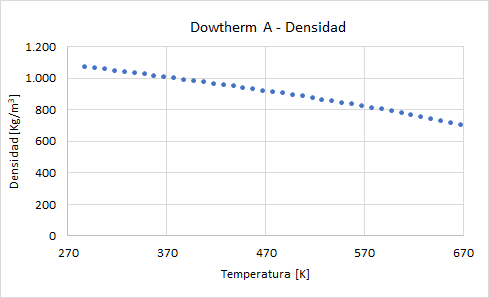
\includegraphics[scale=0.8]{images/curva_densidad.png}
\caption{Densidad en función de la temperatura.} 
\label{fig:curvadensidad}
\end{figure}

\begin{figure}[!h]
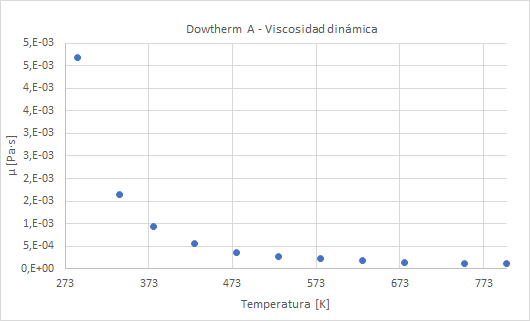
\includegraphics[scale=0.8]{images/curva_viscosidad.png}
\caption{Viscosidad dinámica en función de la temperatura.} 
\label{fig:curvaviscosidad}
\end{figure}

\begin{figure}[!h]
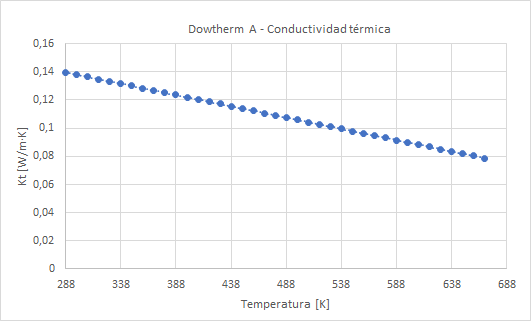
\includegraphics[scale=0.8]{images/curva_conductividad_termica.png}
\caption{Conductividad térmica en función de la temperatura.} 
\label{fig:curvaconductividad}
\end{figure}

\begin{figure}[!h]
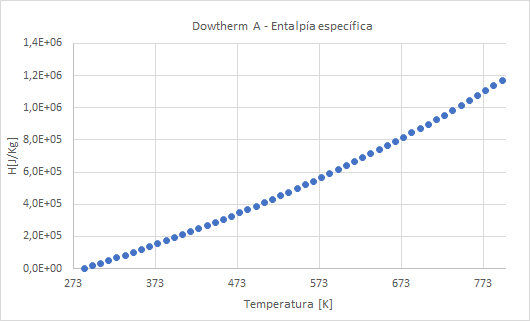
\includegraphics[scale=0.8]{images/curva_entalpia.png}
\caption{Entalpía en función de la temperatura.} 
\label{fig:curvaentalpia}
\end{figure}

\begin{figure}[!h]
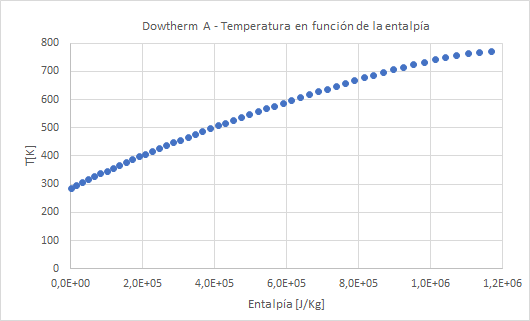
\includegraphics[scale=0.8]{images/curva_temperatura_entalpia.png}
\caption{Temperatura en función de la entalpía.} 
\label{fig:curvatemperatura}
\end{figure}

Para el caso del Dowtherm-A se han obtenido los coeficientes de los polinómios que caracterizan cada parámetro a partir de \cite{richardl.mooreImplementationDOWTHERMProperties2010} y se han contrastado las curvas con los datos ofrecidos en \cite{machadoProductTechnicalData}. En el caso de la viscosidad cinemática se ha detectado que el polinomio de 8º grado que se optiene con los coeficientes de la primera referencia presenta una gran desviación y crecimiento asintótico para temperaturas ligeramente superiores a la máxima de operación del fluido. Con el fin de poder flexibilizar el proceso de cálculo y que no se produzcan desbordamientos se ha ajustado un nuevo polinomio tras extender los datos de la viscosidad dinámica hasta unos 450 °C aproximadamente según la tendencia observada en el último tramo de la curva \(\mu(T)\). De esta forma seobtiene un nuevo polinomio, con mejor comportammiento en este rango extendido.

El mismo procedimiento se ha empleado para obtener los polinomios característicos del fluido Therminol VP-1, aunque en este caso los polinomios se han ajustado a partir de una lista de valores sacada de la librería CoolProp. Pese a que el programa de simulación permite que durante el tiempo de ejecución se obtengan los parámetros citados a través de esta librería, existe una limitación debido al rígido margen de temperaturas con el que esta librería trabaja para cada fluído y esto
provoca que para valores de temperatura ligeramente superiores al rango de operación ofrecido por fabricante no se devuelva ningún valor. Esto resulta en problemas en tiempo de ejecución si algún lazo alcanza una temperatura superior a los 397°C (398°C en el caso de Syltherm 800) . Aunque superar esta temperatura no es recomendable, es algo que puntualmente ocurre durante la operación de la planta. Además, una forma calcular la energía desaprovechada por desenfoque sería a partir de la temperatura que hubiera alcanzado el lazo de no haberse producido el desenfoque y calculando posteriormente su entalpía. Esta aproximación, que sería imposíble en la vida real debido a la degradación del HTF e incluso al daño del propio sistema por las sobrepresiones que se producirían, facilita el cálculo de la energía desaprovechada en cada  momento. Se ha supuesto que las curvas de los parámetros se mantienen bien ajustadas siempre y cuando la sobretemperatura alcanzada no sea excesiva (en las simulaciones realizadas no se ha superado más del 10\% de la temperatura máxima de operación recomendada por el fabricante). Por estos motivos, para este trabajo se han empleado siempre los valores de los parámetros obtenidos a partir de los polinomios y no de CoolProp.

A continuación, en la siguiente tabla, se muestran los coeficientes para Dowtherm A:

Coeficientes de los polinomios de ajuste para Dowtherm A

\begin{longtable}[!h]{@{}lllllll@{}}
& \(C_p(T)\) & \(\mu(T)\) & \(\rho(T)\) & \(k_T(T)\) & \(H(T)\) &
\(T(H)\)\tabularnewline

\endhead
\(a_0\) & -2,363E+03 & 1,583E+00 & 1,492E+03 & 1,856E-01 & -6,511E+05 &
2,853E+02\tabularnewline
\(a_1\) & 3,946E+01 & -2,338E-02 & -3,332E+00 & -1,600E-04 & 4,121E+03 &
6,207E-04\tabularnewline
\(a_2\) & -1,702E-01 & 1,504E-04 & 1,248E-02 & 5,913E-12 & -1,235E+01 &
-1,822E-10\tabularnewline
\(a_3\) & 3,904E-04 & -5,489E-07 & -2,968E-05 & 0 & 2,771E-02 &
-1,423E-16\tabularnewline
\(a_4\) & -4,422E-07 & 1,242E-09 & 3,444E-08 & 0 & -2,776E-05 &
3,316E-22\tabularnewline
\(a_5\) & 1,979E-10 & -1,781E-12 & -1,622E-11 & 0 & 1,106E-08 &
-1,753E-28\tabularnewline
\(a_6\) & 0 & 1,581E-15 & 0 & 0 & 0 & 0\tabularnewline
\(a_7\) & 0 & -7,941E-19 & 0 & 0 & 0 & 0\tabularnewline
\(a_8\) & 0 & 1,728E-22 & 0 & 0 & 0 & 0\tabularnewline

\end{longtable}

Para el caso del Therminol VP-1 los coeficientes son los siguientes:

Coeficientes de los polinomios de ajuste para Therminol VP-1

\begin{longtable}[!h]{@{}lllllll@{}}

& \(C_p(T)\) & \(\mu(T)\) & \(\rho(T)\) & \(k_T(T)\) & \(H(T)\) &
\(T(H)\)\tabularnewline

\endhead
\(a_0\) & 2,881E+02 & 1,487E+00 & 1,403E+03 & 1,486E-01 & -2,923E+05 &
2,924E+02\tabularnewline
\(a_1\) & 5,875E+00 & -2,186E-02 & -1,613E+00 & 9,755E-06 & 3,910E+02 &
6,424E-04\tabularnewline
\(a_2\) & -6,857E-03 & 1,400E-04 & 2,138E-03 & -1,780E-07 & 2,076E+00 &
-3,396E-10\tabularnewline
\(a_3\) & 4,844E-06 & -5,092E-07 & -1,931E-06 & 3,524E-12 & 1,811E-03 &
2,587E-16\tabularnewline
\(a_4\) & 6,960E-20 & 1,148E-09 & -9,610E-21 & -7,572E-25 & -1,089E-05 &
-1,066E-22\tabularnewline
\(a_5\) & -2,780E-23 & -1,642E-12 & 3,864E-24 & 2,948E-28 & 2,274E-08 &
0,000E+00\tabularnewline
\(a_6\) & 0,000E+00 & 1,454E-15 & 0,000E+00 & 0,000E+00 & -2,667E-11 &
0,000E+00\tabularnewline
\(a_7\) & 0,000E+00 & -7,286E-19 & 0,000E+00 & 0,000E+00 & 1,788E-14 &
0,000E+00\tabularnewline
\(a_8\) & 0,000E+00 & 1,583E-22 & 0,000E+00 & 0,000E+00 & -5,284E-18 &
0,000E+00\tabularnewline

\end{longtable}


\subsection{Clases Weather, FieldData y TableData}
\label{clases-weather}
Estas clases impolemetan métodos adecuados para la adquisición de datos desde diferentes tipos de ficheros, en concreto:

\begin{itemize}
\item
  Clase Weather para ficheros .tmy con datos meteorológicos (Weather   Files). En estos ficheros solo hay datos meteorológicos como radiación   normal incidente (DNI), temperatura de bulbo seco, y datos de   geográificos del emplazamiento (Site), como latitud, longitud y   altitud. A partir de estos datos se pueden realizar simulaciones para   ver cuál sería el comportamiento de la planta con estas condiciones.
\item
  Clase FieldData para ficheros .csv con datos recogidos de alguna   planta (Field Data Files). Estos ficheros contienen dastos   meteorológicos recogidos por la estaciones de planta y también datos   de instrumentación de planta, en concreto, temperaturas y presiones de   entrada y salida al campo solar y los diferentes subcampos y también   caudales másicos en los subcampos. Los encabezados de cada columna   probablemente serán identificadores o tags propios de cada planta, por
  lo que es necesario indicar al programa a qué dato corresponde cada   tag. Esto se puede hacer en el fichero de configuracion de la   simulación. Con estos datos se puede simular el comportamiento del   campo solar para caudal teórico requerido pero también comprobar cuál   sería el rendimiento del campo solar operando con el caudal real de  planta. Los datos obtenidos podrán después compararse con los reales   de funcionamiento de planta. A este tipo de simulaciones las   denominaremos `benchmark'.
\item
  Clase TableData para ficheros .csv empleados en simulaciones   distintas, por ejemplo para el estudio del rendimiento de un lazo en   función de diferentes valores de \(q_{abs}\).
\end{itemize}

\hypertarget{clases-site}{Clases Site}

La Clase Site (Emplazamiento), contiene la información relativa al lugar donde está ubicada la planta. Los datos de latitud, longitud y altitud son importantes a la hora de calcular la trayectoria solar para cada fecha. Nos ofrece un método para calcular la posición del sol en cada fecha del año en base a los parámetros que almacenan las coordenadas geográficas. 

\section{Algoritmo de simulación}

En este apartado se describe como puede desarrollarse un código a partir de las Clases implementadas y comentadas anteriormente con el fin de realizar diferentes tipos de simulaciones. Para ello, se continua con la filosofía de POO y se crea desarrolla la clase SolarFieldSimulation.

El objetivo que nos proponemos es simular el comportamiento de un campo solar bajo unas determinadas condiciones. Puesto que estas condiciones varían a lo largo del día, se emplearán ficheros de datos en formato tabular que cuentan con una columna índice para la fecha y hora indicadas. Con el fin de poder reaprovechar el trabajo realizado durante el trabajo de configuración de la simulación, se emplea un archivo en formato JSON que recoge todos los parámetros necesarios. En resumen, la instancia de SolarFieldSimulation recibe realiza los siguientes pasos:

\begin{itemize}
\item
  Lee el archivo de configuración de la simulación y almacena los   parámetros necesarios.
\item
  Crea una instancia de la Clase Site con información sobre la ubicación   de la planta.
\item
  Crea una instancia para el almacenamiento de los datos del fichero en   formato tipo tabla. En función de si el fichero es de tipo   meteorológico (TMY2 o TMY3) o es un fichero en formato CSV creará una   instancia de la clase Weather o FieldData respectivamente. Los datos   cargados se almacenan en un DataFrame de la librería Pandas denominado  \emph{datasource}.
\item
  Crea una instancia para el modelado del HTF a partir de la Clase   FluidCoolProp si los datos se van a tomar desde la libería externa   CoolProp o de la Clase FluidTabular si se le pasan los factores de los   polinomios que permiten calcular cada parámetro del fluido.
\item
  Crea una instancia SolarField a partir de los parámetros de   configuración de campo solar.
\item
  Crea una instancia BaseLoop a partir de los parámetros de   configuración de lazo.
\end{itemize}

A partir de aquí, la instancia de SolarFieldSimulation ya dispone de lo necesario para realizar la simulación del campo mediante su método \emph{runSimulation()}.

El tipo de simulación que se realiza depende del tipo de datos de que se disponga y de lo que se seleccione en el archivo de configuración:

\begin{itemize}
\item
  Simulación tipo \emph{simulation}: En este caso, el caudal del lazo se   recalculará en un proceso de convergencia hasta conseguir que la   temperatura de salida del lazo sea la temperatura consignada.

  \begin{itemize}
  \item
    Si el tipo de datos del que se dispone no tiene datos reales de  planta, la instancia \emph{datasource} será de tipo Weather y solo   se cuenta con datos meteorológicos (\(DNI\), \(T_{ext}\), velocidad
    del viento y presión atmosférica), por lo que la temperatura de   entrada a los lazos será la nominal
  \item
    Si el tipo de datos del que se dispone sí cuenta con datos reales de   planta que permitan conocer las temperaturas de entrada a los lazos  (como es nuestro caso), la simulación utilizará estas temperaturas a  la hora de ajustar los caudales al salto térmico necesario.
  \end{itemize}
\item
  Simualción tipo \emph{benchmark}: En este caso se debe disponer  obligatoriamente de datos reales de planta, pues la simulación utiliza  las temperaturas de entrada a los lazos y los caudales reales para calcular cúal será la temperatura de salida. Posteriormente, en los  archivos de salida de datos, se puede comparar la temperatura real de  salida del lazo con la calculada y de esta forma estimar si ha habido desenfoque y por tanto, desaprovechamiento de la energía solar. Hay
  que tener en cuenta en los datos que disponemos podemos encontrar   situaciones en las que el lazo alcanza su temperatura de consigna pero   es posible que se estuviera realizando un ajuste de enfoque-desenfoque   (ya que el caudal no es regulable a nivel de lazo). En ese caso, es   intersante saber qué temperatura hubera alcanzado el HTF de no haberse   producido el desenfoque y, por tanto, poder calcular la energía solar   que no se ha aprovechado por no poder introducir mayor caudal en el   lazo.
\end{itemize}

A la hora de realizarse cada una de estas simulaciones puede darse el caso de que se haya configurado la opción \emph{fastmode=True}. En este caso se considera que todos los lazos de la planta se comportan como el lazo típico, modelado mediante la Clase BaseLoop. En caso contrario, la simulación se realizará para cada lazo del campo, lo cual solo tiene sentido si los lazos o sus componentes cuentan con diferentes valores en sus parámetros. 

Una vez que el método runSimulation() ha procesado todas las filas seleccionadas del DataFrame \emph{datasource}, los datos calculados que se han ido añadiendo al DataFrame son volcados a un archivo CSV para su posterior análisis.

\subsection{Simulación tipo simulation}

Tal y como se ha mencionado, en este caso se simula la planta de tal forma que se calcula el caudal necesario en cada lazo con el fin de que se alcance la temperatura de consigna o nominal. En este tipo de simulación solo son necesarios los datos meteorológicos y los valores nominales de temperatura y presión de entrada y salida. Los valores exactos de la presión no son necesarios y basta con seleccionar presiones suficientemente altas para que garanticen el estado de líquido
saturado del HTF en todo momento. Las propiedades del HTF en estado de líquido saturado no dependen significativamente de la presión.

Los datos meteorológicos se pueden leer de un fichero en formato TMY2, TMY3 o CSV convenientemente etiquetado. Si además se dispone de los datos de temperatura de entrada del HTF al campo solar se emplearán éstos en lugar del valor nominal, por lo que el salto térmico necesario se calculará partiendo de la temperatura real de entrada.

El programa calcula el rendimiento del lazo base o de cada lazo (según se haya seleccionado o no la opción \emph{fastmode}) ajusando iterativamente el caudal hasta que la temperatura de salida sea la consignada. Durante las horas nocturnas el caudal es fijo e igual al mínimo recomendado, tal y como ocurre en plantas reales. 

\hypertarget{simulaciuxf3n-tipo-benchmark}{Simulación tipo benchmark}

En este tipo de simulación el caudal viene marcado por el caudal real de planta, por lo que para este tipo de simulación es obligatorio disponer de los datos reales. Al emplearse un caudal fijo, la temperatura alcanzada por el HTF en la simulación no tiene porqué coincidir con la temperatura real. Dependiendo de si el valor obtenido es mayor o menor que el real se pueden sacar las siguientes interpretaciones: 
* Si la  temperatura calculada es menor que la real podemos interpretar que la simulación ha sobredimensionado las pérdidas en la configuración de la planta. Pueden corregirse algunos parámetros o introducir un factor multiplicativo. 
* Si la temperatura calculada es mayor que la real puede deberse a que se han infravalorado las pérdidas, lo cual se podría corregir ajustando los valores de estas en el archivo de configuración, pero también puede deberse a que el campo real estaba realizando desenfoques parciales para reducir la energía captada. En ese caso, la energía no aprovechada se puede calcular como la diferencia entre la entalpía del HTF a la temperatura de salida simulada menos su entalpia a la temperatura de salida real.

\section{Validación por comparación con otra herramienta de simulación}

Con el fin realizar una primera validación de nuestro código, compararemos en primer lugar los valores obtenidos para una determinada configuración de campo con los que se optienen mediante System Advisor Model (SAM, \cite{freemanSystemAdvisorModel2018}), un software de reconocido prestigio muy empleado en el sector de las energía renovables. Las posibilidades de SAM van mucho más allá del alcance de nuestro código, pudiendo realizar el modelado no solo de sistemas de energía solar de concentración sino también de sistemas fotovoltaicos, geotérmicos, mareomotrices, eólicos, de biomasa por ejemplo. Dentro de los sistemas de energía solar térmica de concentración, ofrece la posibilidad de modelar centrales de las cuatro principales tecnologías ya comentadas y a su vez, de diversas variedades. SAM realiza también el análisis económico y financiero del proyecto basándose principalmente en la generación eléctrica que se espera generar. Por este motivo, SAM tiene en cuenta el acoplamiento del campo solar con el bloque de potencia a la hora de realizar la simulación.  Esto hace que no podamos comparar directamente nuestro programa con los modelos de SAM para genaración eléctrica, pues los ajustes que hace SAM afectan al comportamiento del campo, introduciendo limitaciones de caudal de HTF y de potencia térmica transferida al bloque de potencia, desenfoques en el campo, rampas de arranque e inercias del sistema que quedan fuera de nuestro alcance. En cambio, SAM también cuenta con un móduo para la simulación de un sistema de generación de calor  para proceso industrial (IPH, Industrial Process Heat) basado en el modelo Físico que emplea para la simulación de plantas CCP. Emplearemos este módulo para comparar los resultados de SAM con nuestro simulador tal y como ese explica a continuación.

\subsection{Configuración de las simulaciones}
\label{configuracion-simulaciones}

Para que una simulación realizada con el módulo IPH de SAM sea comparable a la nuestra indicaremos que no existe almacenamiento térmico para evitar procesos de mezcla de HTF a diferentes temperaturas que se producirían en ese caso. También indicaremos que el sumidero térmico tiene capacidad elevada, lo que, en principio, nos obligaría a seleccionar un tamaño de campo solar muy grande. Para que el tamaño de campo solar sea igual al del campo que queremos simular indicaremos a SAM que las condiciones de radiación solar nominales son mucho más elevadas que las que se alcanzarán en cualquier momento el año $(2000 W/m^2)$. De este modo conseguimos que el dimensionado que hace SAM del campo solar sea igual que el nuestro (120 lazos), pero que no se produzca desenfoque en ningún momento. Es decir, con SAM extraemos del campo solar toda energía posible, al igual que hace nuestro simulador.

Puesto que solo modelamos el campo, no tenemos a priori ninguna información sobre la temperatura de retorno del HTF frío desde el intercambiador donde cede su energía al sumidero térmico. Con el fin de que la comparación sea lo más ajustada posible, aprovecharemos los datos de temperatura de HTF frío que se optienen de la simulación de SAM como datos de entrada para nuestra simulación. De esta forma, en ambas simulaciones el salto térmico se realiza desde el mismo punto de partida. Además, indicaremos a SAM que no existe inercia térmica en tuberías y concentradores y prescindiremos del cálculo de pérdidas térmicas en las primeras.

Respecto al fluído caloportador, SAM nos permite seleccionar entre una serie de fluidos preconfigurados. Seleccionaremos Therminol VP-1 pues también podemos simular este fluido con nuestro programa.

Realizaremos la simulación para un año completo. Contamos con los datos meteorológicos del año 2007 en formato TMY3.  En la Fig.\ref{fig:captura01} se puede ver la pestaña de configuración de SAM para seleccionar el origen de datos meteorológicos.

\begin{figure}[!h]
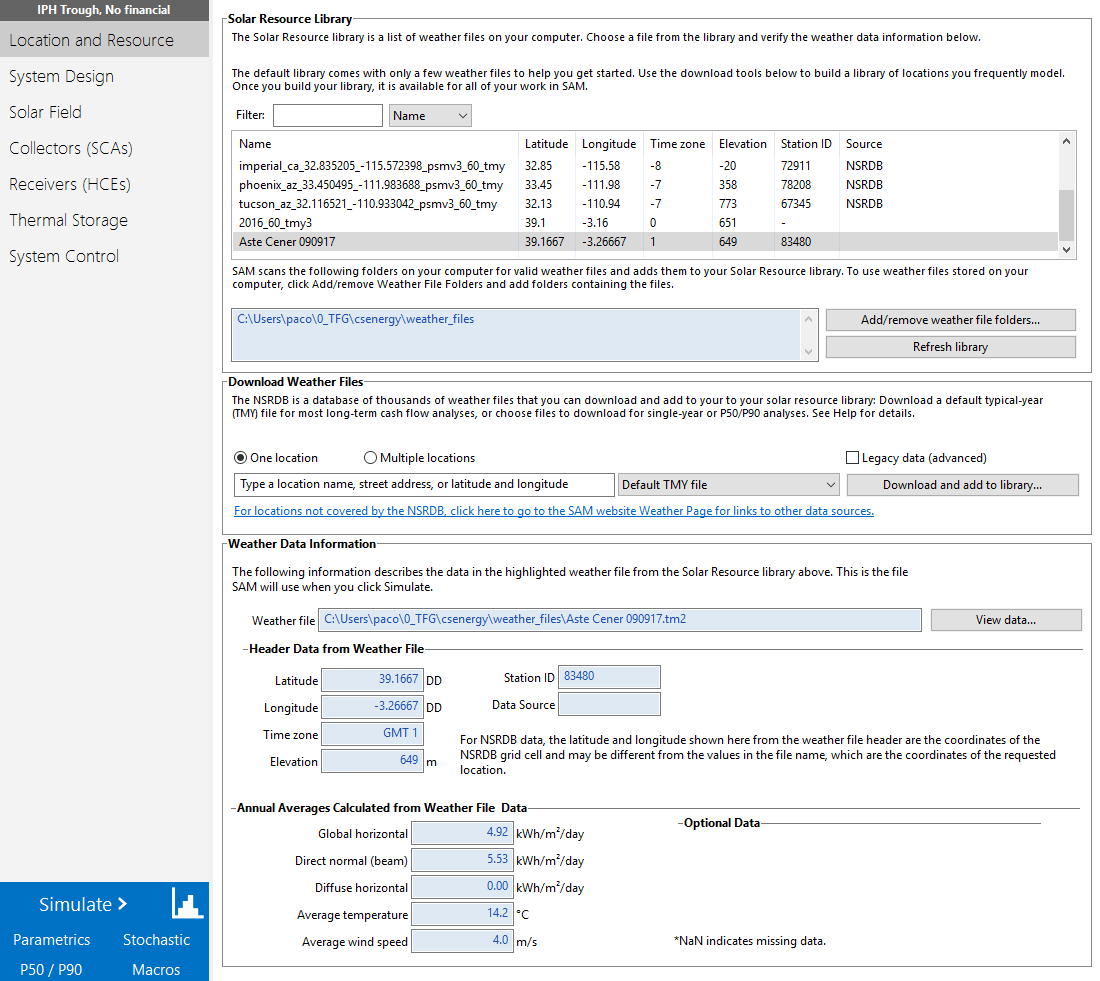
\includegraphics[width=0.9\linewidth]{images/captura_sam_iph01.png}
\caption{Configuración SAM. Seleccción del archivo de datos meterorológicos} 
\label{fig:captura01}
\end{figure}


La versión de SAM utilizada ha sido la \emph{''2020.2.29, 64 bit, updated to revision 1''}. En la Fig.\ref{fig:captura02} podemos ver la pestaña de configuracion del campo solar. 

\begin{figure}[!h]
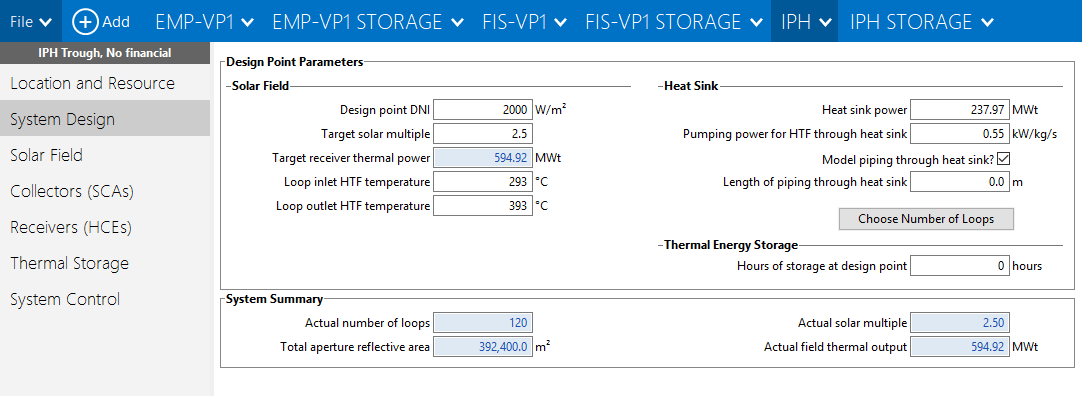
\includegraphics[width=0.9\linewidth]{images/captura_sam_iph02.png}
\caption{Configuración SAM. Campo solar} 
\label{fig:captura02}
\end{figure}

Los SCA, modelo SenerTrough I diseñado por Sener, se han parametrizado de la siguiente manera a partir del modelo EuroTrough ET150:

\begin{table}[!h]
\centering
\caption{Configuración del SCA modelo SenerTrough I de Sener}
\label{tab:configuracionSCA}
\begin{tabular}{lc}
Parámetro & Valor \\ \hline
Longitud &  148,5  (m) \\
Apertura &  5,77  (m) \\
Distancia Focal & 2,1 (m) \\
Coeficiente $F_{0}$ del  IAM  &  1 \\
Coeficiente $F_{1}$ del  IAM  &  0,0506 \\
Coeficiente $F_{2}$ del  IAM  &  -0,1763 \\
Precisión del seguidor &  0,99 \\
Precisión geométrica &  0,98 \\
Disponibilidad &  0,99 \\
Reflectividad &  0,935 \\
Limpieza &  0,98
\end{tabular}
\end{table}


En la Fig.\ref{fig:captura03} puede verse una captura de pantalla de la pestaña de configuración del tipo de SCA en SAM. En la Fig.\ref{fig:capture04}, puede verse la pestaña correspondiente a la configuración de HCE. En este caso el modelo empleado es el UVAC 3, de Solel, con los parámetros que se indican en la \ref{tab:configuracionHCE}.


\begin{figure}[!h]
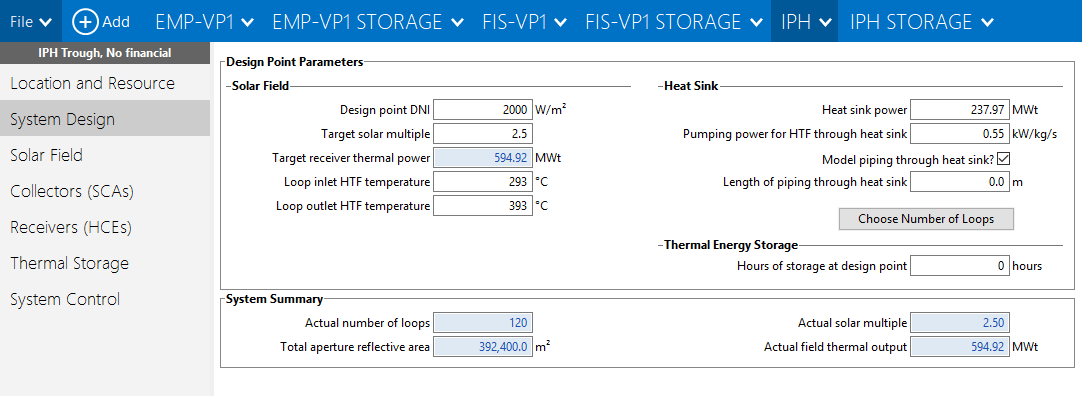
\includegraphics[width=0.9\linewidth]{images/captura_sam_iph02.png}
\caption{Configuración SAM. Configuración del SCA SenerTrough I a partir del modelo EuroTrough ET150} 
\label{fig:captura03}
\end{figure}

\begin{figure}[!h]
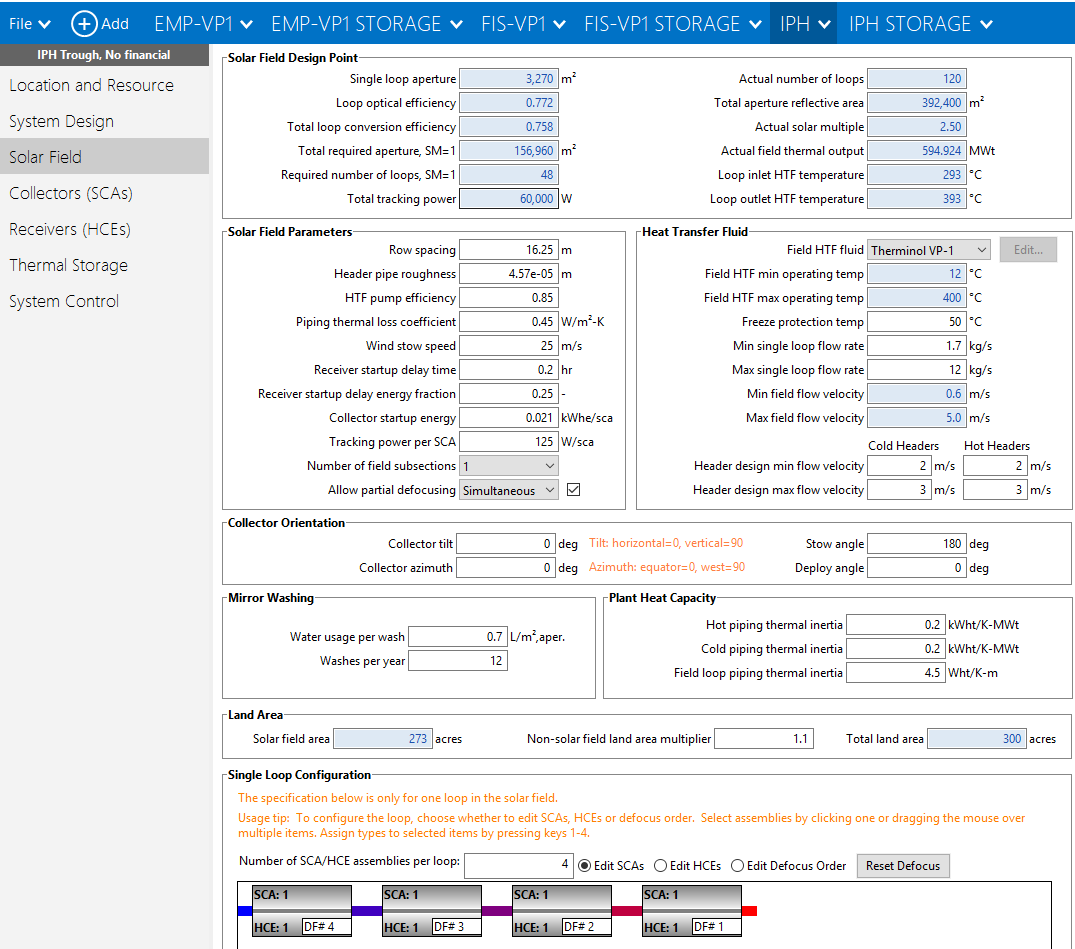
\includegraphics[width=0.9\linewidth]{images/captura_sam_iph03.png}
\caption{Configuración SAM. Configuración del HCE UVAC 3 con vacío}
\label{fig:captura04}
\end{figure}


\begin{table}[!h]
\centering
\caption{Configuración del HCE modelo UVAC 3 de Solel}
\label{tab:configuracionHCE}
\begin{tabular}{lc}
Parámetro & Valor \\ \hline
Logintud & 4,05 (m) \\
Factor de longitud efectiva, \(\gamma_L\) &  0,96 \\
Factor de interceptación geométrica, \(\gamma_g\) & 0,96 \\
Diámetro interior del tubo absorbedor, \(d_{ri}\) & 0,066 (m) \\
Diámetro exterior del tubo absorbedor, \(d_{ro}\)r &  0,070 (m) \\ 
Diámetro interior de la envolvente de vídrio, \(d_{gi}\) &  0,115 (m) \\
Diámetro exterior de la envolvente de vídrio, \(d_{go}\) &  0,121 (m) \\
Rugosidad interior &  0,000045 (m)  \\
Factor de emisividad, \(A_1\) &  0,000206 \\
Factor de emisividad, \(A_0\) &  0,0430 \\
Absortibidad solar del receptor &  0,96 \\
Transmisividad del vídrio &  0,96 \\
Valor mínimo del número de Reynolds recomendado &  2300 \\
Distancia de separación entre brazos de soportación &  4,05 (m) 
\end{tabular}
\end{table}

Se ha considerado que todos los HCE  del campo se encuentran en buen estado de vacío.

Para la configuración de la simulación con nuestro código se debe crear un archivo en formato JSON con el que se le pasa toda la información necesaria. Con el fin de facilitar la creación de este archivo de configuración se ha desarrollado una sencilla interfaz que sirve de guía durante el proceso. En la Fig.\ref{fig:interface01} se muestra la primera pantalla de la interfaz de configuración. El archivo de origen de datos incluye los mismos datos meteorológicos que se han empleado para SAM y, además, los datos de temperatura de entrada del HTF al campo solar que ha generado SAM en la simulación IPH. También emplearemos el caudal calculado por SAM para compararlo con el que calcula nuestro simulador.

\begin{figure}[!h]
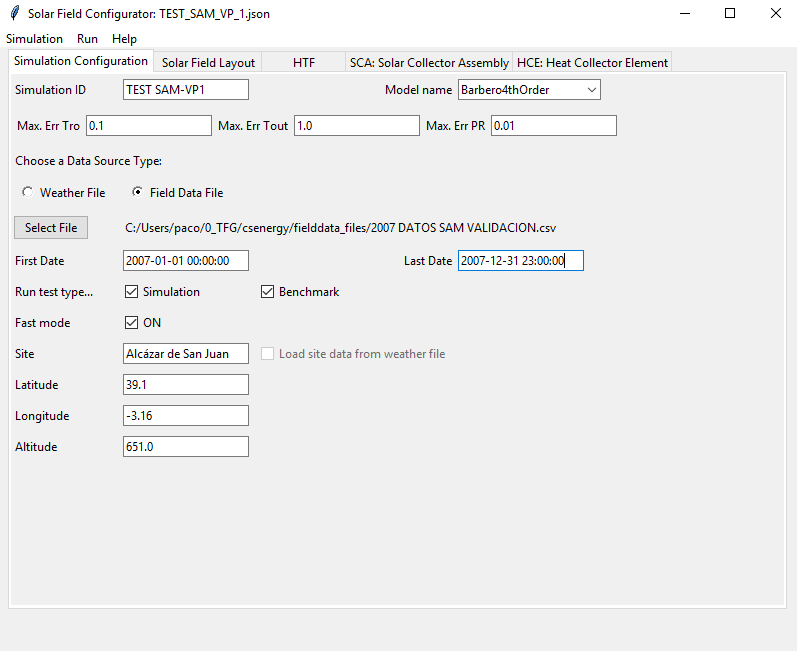
\includegraphics[width=0.9\linewidth]{images/interface01.png}
\caption{Configuración de la simulación. Selección del tipo de simulación, fichero de datos y lugar de emplazamiento.} 
\label{fig:interface01}
\end{figure}

La configuración del campo solar es similar a la de SAM. Con el fin acelerar el proceso de simulación, consideraremos que hay 2 HCEs en cada SCA. Es decir, cada HCE tiene una longitud de 72,9 m, que está por debajo del límite de 100 m que nos hemos impuesto como criterio de validez del tamaño de malla para el modelo unidimensional.  El caudal mínimo de recirculación en cada lazo es de 1,7 kg/s. La temperatura de salida deseada es de $393\circ C$ (666,15 K).

\begin{figure}[!h]
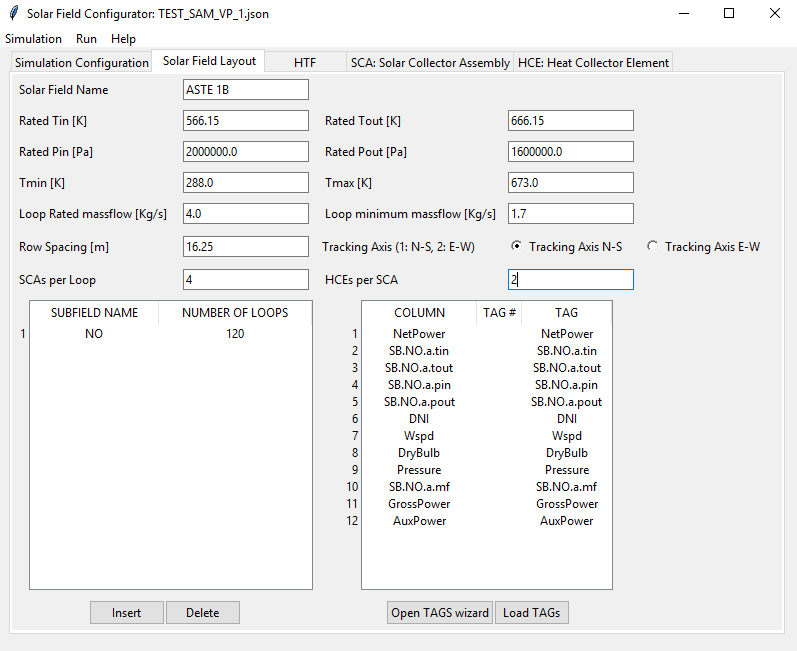
\includegraphics[width=0.9\linewidth]{images/interface02.png}
\caption{Configuración de la simulación. Configuración del campo solar, número de subcampos, lazos, configuración de los lazos, valores nominales y asistente para relacionar los identificadores de las columnas del archivo de origen de datos con los que maneja el programa.} 
\label{fig:interface02}
\end{figure}

El fluido caloportador Therminol VP-1 se configura tal y como puede verse en la Fig.\ref{fig:interface03}. Los coeficientes se cargan desde una librería donde los hemos guardado previamente tras su obtención según se indicó en el apartado \ref{subclases-fluid}.

\begin{figure}[!h]
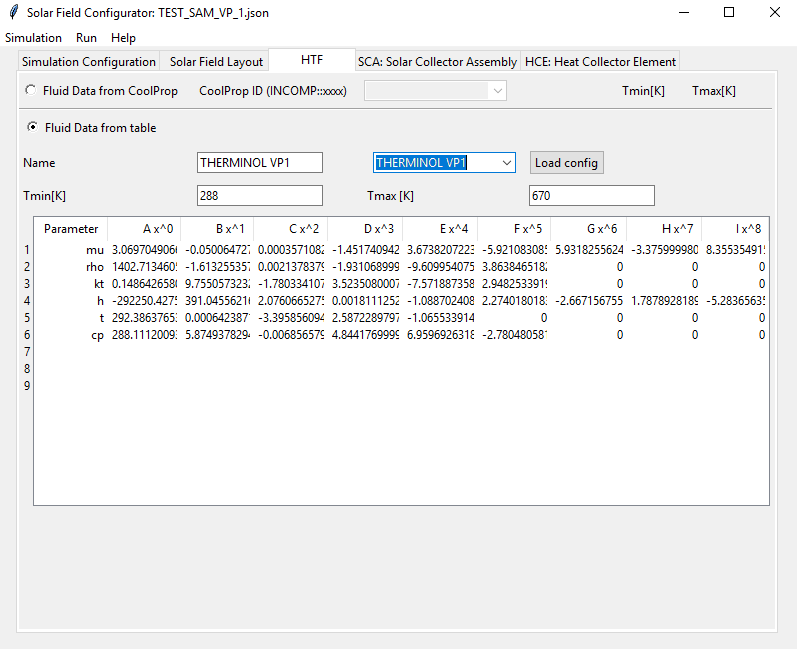
\includegraphics[width=0.9\linewidth]{images/interface03.png}
\caption{Configuración de la simulación. Selección y configuración del fluido caloportador} 
\label{fig:interface03}
\end{figure}

Finalmente, en las figuras \ref{fig:interface04} y \ref{fig:interface05} puede verse la configuración del tipo de SCA y HCE respectivamente.

\begin{figure}[!h]
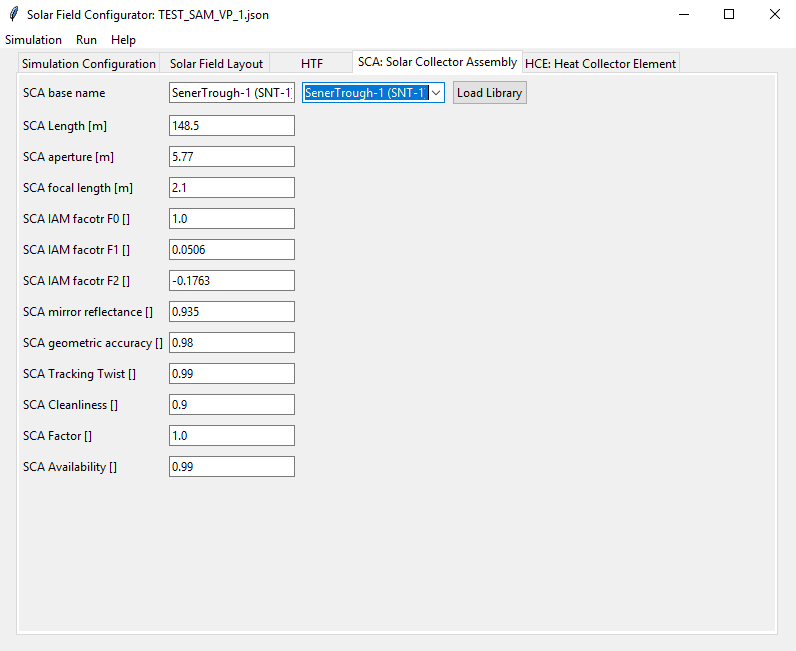
\includegraphics[width=0.9\linewidth]{images/interface04.png}
\caption{Configuración de la simulación. Selección del modelo de SCA y configuración} 
\label{fig:interface04}
\end{figure}

\begin{figure}[!h]
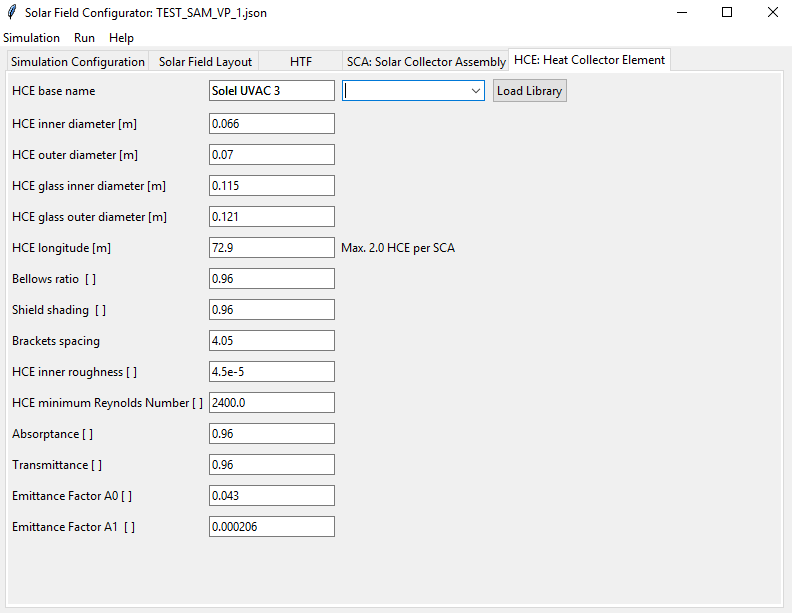
\includegraphics[width=0.9\linewidth]{images/interface05.png}
\caption{Configuración de la simulación. Selección del modelo de HCE y configuración} 
\label{fig:interface05}
\end{figure}

\subsection{Resultados de la validación}
\label{resultados-validacion}
 
Una vez que tenemos configurado SAM y nuestro programa de la misma manera ejecutamos SAM sobre un archivo con los datos meteorológicos de un año y en valores horarios, en concreto se trata de los datos del año 2009 que se emplearon para el estudio y anteproyecto de construcción de las plantas.  

En el campo solar de 120 lazos, con una superfice total de captación de 392400 $m^2$ la energía anual incidente es de 792,1 GWh, que se ve reducida a 686,4 GWh debido a que el ángulo de incidencia es distinto de cero (efecto coseno).

En la Tabla \ref{tab:energia_anual} se muestran los valores  calculados por SAM y los que obtenemos con nuestro código. SAM denonima ''Receiver thermal power incident'' a la radiación solar que finalmente alcanza al fluido caloportador, es decir, la radaciación solar incidente menos las pérdidas ópticas. Este valor es equivalente a lo que nosotros hemos venido denominando ''potencia absorbida, $\cdot q_{abs}$''. 

\begin{table}[!h]
\centering
\caption{Resultados globales anuales para las simulaciones con SAM y Python}
\label{tab:generacion_anual}
\begin{tabular}{lcc}
Valores anuales  & SAM & Código Python \\ \hline
Potencia incidente (GWh/año)	& 686		& 686			\\ 
Potencia absorbida (GWh/año)	& 477		& 491			\\ 
Rencimiento óptico 			& 0,695	 	& 0,716			\\ 
Pérdidas térmicas (GWh/año)	& 64		& 73			\\ 
Rendimiento térmico			& 0,866		& 0,851			\\ 
Potencia térmica (GWh/año) 	& 413		& 418	        	\\ 
\end{tabular}
\end{table}

Comprobamos que existe una ligera desviación en el rendimiento óptico anual (2,9\%) y en el rendimento térmico anual (1,9\%). El origen de esta desviación se encuentra en la dificultad de adaptar exactametne la configuracón de nuestra simulación a la de SAM pues no todos los parámetros son equivalentes en ambas casos. Por otro lado, por tratarse de valores anuales, existe una acumulación de pequeñas desviaciones que se producen entre ambas simulaciones, principalmente a primera y última hora del día  y durante jornadas de gran inestabilidad en la radiación. 

Nos fijaremos ahora en el comportamiento para varios días del año. Hemos seleccionado un día de gran estabilidad y buena radiación solar y otro día menos estable y con peores condiciones. En las figuras \ref{fig:177caudal}  a \ref{fig:177temperatura} podemos ver la evolución del caudal, la temperatura y la potencia térmica en ambas simulaciones para el día 17 de julio (buenas condiciones de radiación y estabilidad). En las figuras \ref{fig:176caudal}  a \ref{fig:176temperatura} podemos ver la evolución para el día 17 de junio, con peores condiciones tal y como se aprecia por los altibajos que presentan las curvas a lo largo del día. En todas las gráficas se ha representado DNI en el eje secundario.

\begin{figure}[!h]
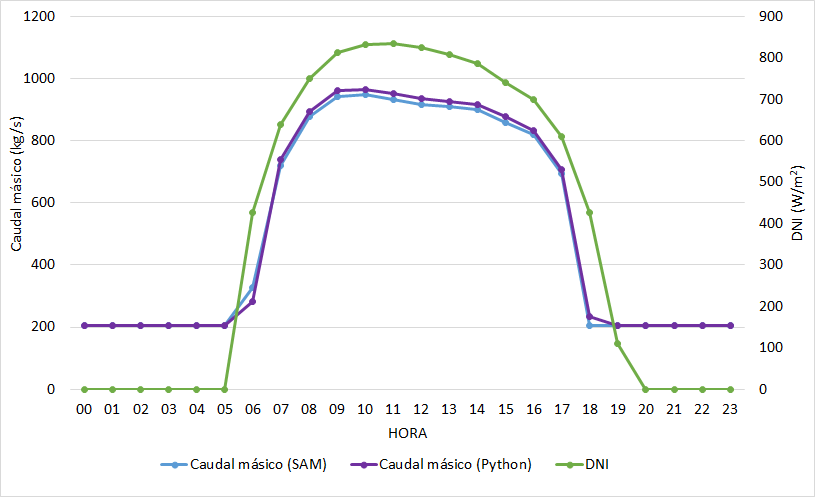
\includegraphics[width=0.9\linewidth]{images/177caudal.png}
\caption{Caudal másico calculado por SAM y por el código Python para el día 17/07/2009} 
\label{fig:177caudal}
\end{figure}

\begin{figure}[!h]
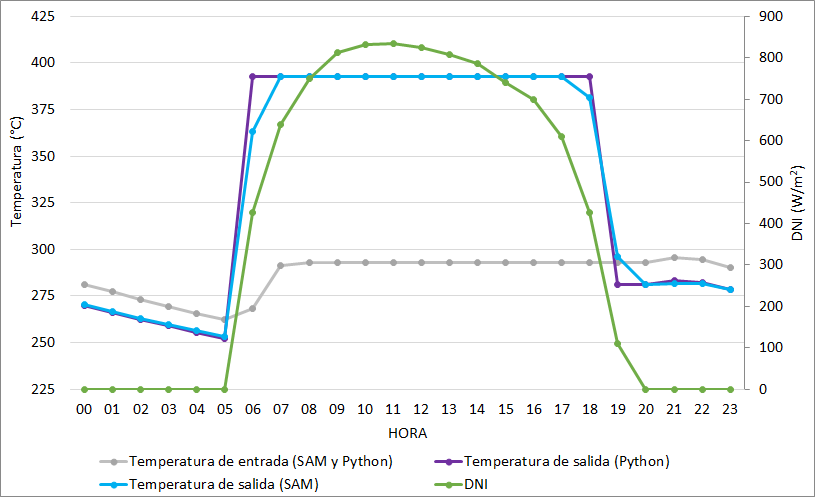
\includegraphics[width=0.9\linewidth]{images/177temperatura.png}
\caption{Temperatura de entrada y de salida calculadas por SAM y por el código Python para el día 17/07/2009} 
\label{fig:177temperatura}
\end{figure}

\begin{figure}[!h]
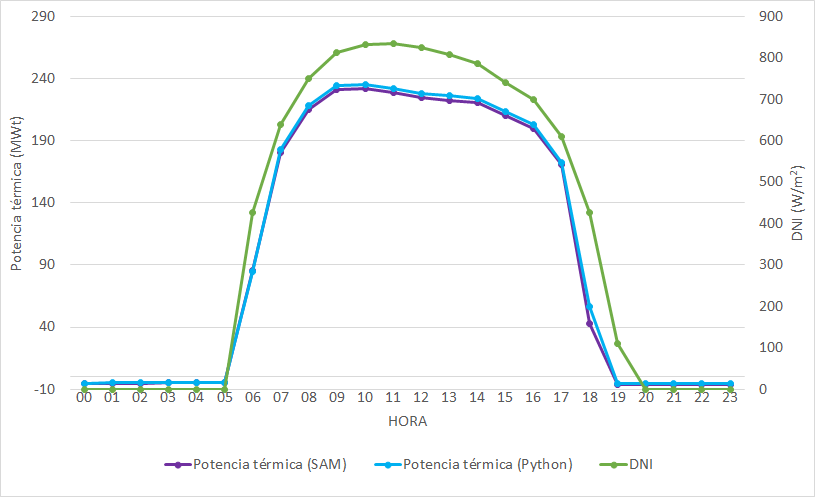
\includegraphics[width=0.9\linewidth]{images/177potencia.png}
\caption{Potencia térmica calculada por SAM y por el código Python para el día 17/07/2009} 
\label{fig:177potencia}
\end{figure}

\begin{table}[!h]
\centering
\caption{Resultados de las simulaciones (S: SAM, P: Python) para el día 17 de julio de 2009. Condiciones estables}
\label{tab:datos_17_julio}
\resizebox{\textwidth}{!}{%
\begin{tabular}{ccccccccc}
Hora &
\parbox{5em}{\centering DNI (S, P) \\ ($W/m^2$)} &
\parbox{5em}{\centering Caudal (S)  \\  ($Kg/s$)}    &
\parbox{5em}{\centering Caudal (P)  \\  ($Kg/s$)}  &
\parbox{5em}{\centering $T_{in}$ (S, P)  \\ $(^\circ C)$} &
\parbox{5em}{\centering $T_{out}$ (S)  \\ $(^\circ C)$} &
\parbox{5em}{\centering $T_{out}$ (P)  \\ $(^\circ C)$} &
\parbox{5em}{\centering Pot. Térmica (S)  \\  (MWt)}  &
\parbox{5em}{\centering Pot. Térmica (P) \\  (MWt)} \\ \hline
0:00  & 0   & 204,0 & 204,0 & 281,3 & 270,4 & 270,0 & -5,5  & -5,2  \\
1:00  & 0   & 204,0 & 204,0 & 277,2 & 266,6 & 266,2 & -5,3  & -5,0  \\
2:00  & 0   & 204,0 & 204,0 & 273,3 & 263,1 & 262,5 & -5,1  & -4,8  \\
3:00  & 0   & 204,0 & 204,0 & 269,5 & 259,6 & 259,0 & -4,9  & -4,7  \\
4:00  & 0   & 204,0 & 204,0 & 265,8 & 256,2 & 255,6 & -4,7  & -4,6  \\
5:00  & 0   & 204,0 & 204,0 & 262,3 & 253,0 & 252,3 & -4,6  & -4,4  \\
6:00  & 426 & 326,4 & 282,9 & 268,5 & 363,0 & 392,7 & 85,7  & 84,5  \\
7:00  & 639 & 721,1 & 739,0 & 291,4 & 392,6 & 392,9 & 180,1 & 182,8 \\
8:00  & 750 & 876,3 & 894,9 & 292,9 & 392,8 & 392,9 & 215,2 & 218,3 \\
9:00  & 812 & 943,4 & 961,0 & 293,0 & 392,5 & 392,9 & 230,7 & 234,3 \\
10:00 & 831 & 947,0 & 964,8 & 293,0 & 392,5 & 392,9 & 231,6 & 235,2 \\
11:00 & 834 & 933,5 & 951,8 & 293,0 & 392,6 & 392,9 & 228,4 & 232,0 \\
12:00 & 825 & 917,1 & 935,7 & 293,0 & 392,6 & 392,9 & 224,6 & 228,1 \\
13:00 & 809 & 908,3 & 926,8 & 293,0 & 392,7 & 392,9 & 222,6 & 225,9 \\
14:00 & 787 & 899,1 & 917,5 & 293,0 & 392,7 & 392,9 & 220,4 & 223,6 \\
15:00 & 740 & 857,7 & 876,1 & 293,0 & 392,9 & 392,9 & 210,6 & 213,5 \\
16:00 & 699 & 818,2 & 831,4 & 293,0 & 392,5 & 392,9 & 200,1 & 202,7 \\
17:00 & 610 & 694,2 & 706,8 & 293,0 & 392,9 & 392,9 & 170,5 & 172,3 \\
18:00 & 426 & 204,0 & 232,5 & 293,0 & 381,4 & 392,9 & 43,1  & 56,7  \\
19:00 & 109 & 204,0 & 204,0 & 293,0 & 295,9 & 281,0 & -6,4  & -5,6  \\
20:00 & 0   & 204,0 & 204,0 & 293,0 & 280,9 & 281,0 & -6,2  & -5,6  \\
21:00 & 0   & 204,0 & 204,0 & 295,7 & 281,4 & 283,5 & -6,3  & -5,7  \\
22:00 & 0   & 204,0 & 204,0 & 294,6 & 281,9 & 282,5 & -6,3  & -5,6  \\
23:00 & 0   & 204,0 & 204,0 & 290,5 & 278,6 & 278,6 & -6,0  & -5,5 
\end{tabular}%
}
\end{table}

\begin{figure}[!h]
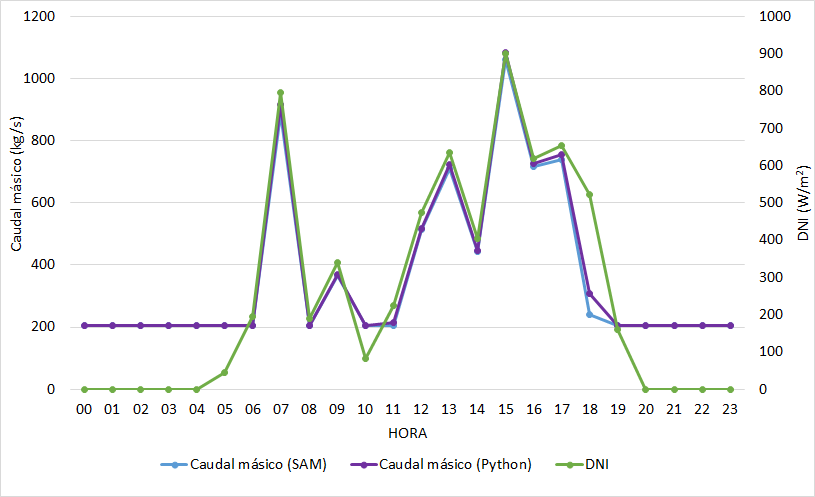
\includegraphics[width=0.9\linewidth]{images/176caudal.png}
\caption{Caudal másico calculado por SAM y por el código Python para el día 17/06/2009} 
\label{fig:176caudal}
\end{figure}

\begin{figure}[!h]
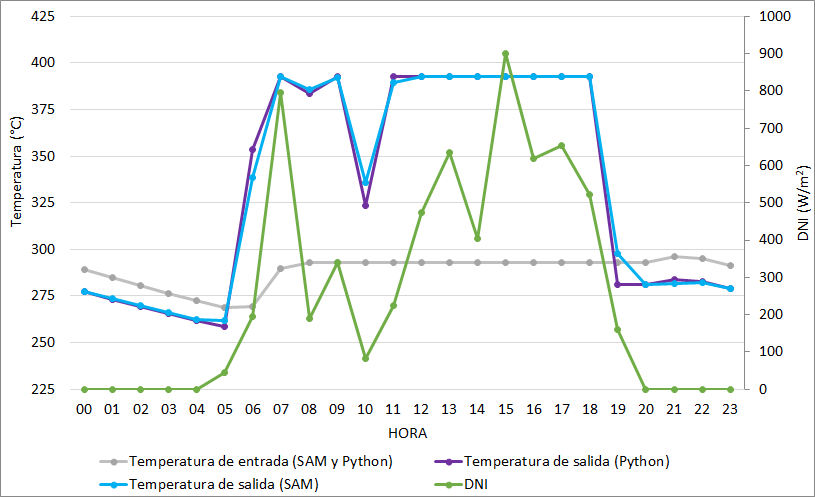
\includegraphics[width=0.9\linewidth]{images/176temperatura.png}
\caption{Temperatura de entrada y de salida calculadas por SAM y por el código Python para el día 17/06/2009} 
\label{fig:176temperatura}
\end{figure}

\begin{figure}[!h]
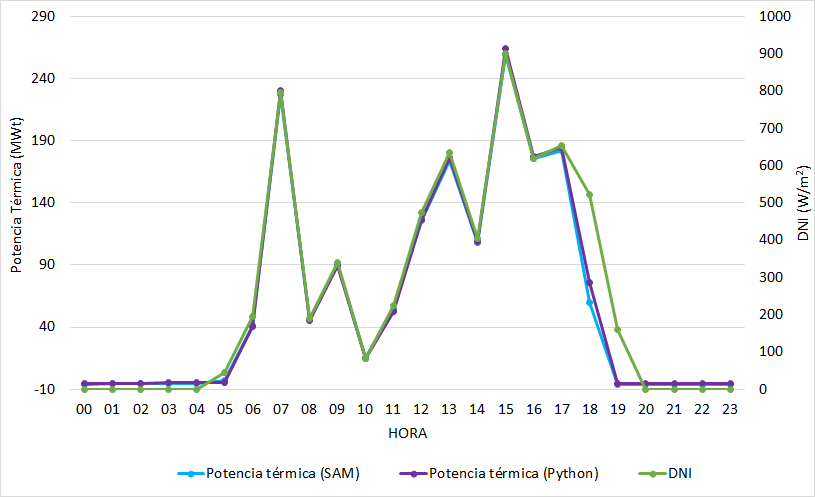
\includegraphics[width=0.9\linewidth]{images/176potencia.png}
\caption{Potencia térmica calculada por SAM y por el código Python para el día 17/06/2009} 
\label{fig:176potencia}
\end{figure}


\begin{table}[!h]
\centering
\caption{Resultados de las simulaciones (S: SAM, P: Python) para el día 17 de junio de 2009. Condiciones inestables}
\label{tab:datos_17_junio}
\resizebox{\textwidth}{!}{%
\begin{tabular}{ccccccccc}
Hora &
\parbox{5em}{\centering DNI (S, P) \\ ($W/m^2$)} &
\parbox{5em}{\centering Caudal (S)  \\  ($Kg/s$)}    &
\parbox{5em}{\centering Caudal (P)  \\  ($Kg/s$)}  &
\parbox{5em}{\centering $T_{in}$ (S, P)  \\ $(^\circ C)$} &
\parbox{5em}{\centering $T_{out}$ (S)  \\ $(^\circ C)$} &
\parbox{5em}{\centering $T_{out}$ (P)  \\ $(^\circ C)$} &
\parbox{5em}{\centering Pot. Térmica (S)  \\  (MWt)}  &
\parbox{5em}{\centering Pot. Térmica (P) \\  (MWt)} \\ \hline
0:00  & 0   & 204,0  & 204,0  & 289,3 & 277,5 & 277,4 & -6,0  & -5,5  \\
1:00  & 0   & 204,0  & 204,0  & 284,8 & 273,5 & 273,3 & -5,8  & -5,3  \\
2:00  & 0   & 204,0  & 204,0  & 280,6 & 269,6 & 269,3 & -5,5  & -5,1  \\
3:00  & 0   & 204,0  & 204,0  & 276,5 & 265,9 & 265,5 & -5,3  & -5,0  \\
4:00  & 0   & 204,0  & 204,0  & 272,5 & 262,3 & 261,8 & -5,1  & -4,8  \\
5:00  & 45  & 204,0  & 204,0  & 268,8 & 262,0 & 258,4 & -3,2  & -4,7  \\
6:00  & 194 & 204,0  & 204,0  & 269,2 & 338,7 & 353,3 & 41,5  & 40,3  \\
7:00  & 795 & 885,8  & 916,9  & 289,7 & 392,7 & 392,9 & 227,1 & 230,5 \\
8:00  & 189 & 204,0  & 204,0  & 292,8 & 385,9 & 383,5 & 46,1  & 44,9  \\
9:00  & 339 & 366,8  & 367,7  & 292,9 & 392,2 & 392,9 & 90,0  & 89,7  \\
10:00 & 81  & 204,0  & 204,0  & 293,0 & 336,0 & 323,7 & 15,6  & 14,7  \\
11:00 & 225 & 204,0  & 215,4  & 293,0 & 389,6 & 392,9 & 53,8  & 52,5  \\
12:00 & 473 & 514,8  & 518,7  & 293,0 & 392,6 & 392,9 & 125,8 & 126,4 \\
13:00 & 634 & 711,7  & 722,5  & 293,0 & 392,5 & 392,9 & 174,1 & 176,1 \\
14:00 & 403 & 442,9  & 445,2  & 293,0 & 392,5 & 392,9 & 108,4 & 108,5 \\
15:00 & 899 & 1059,6 & 1082,5 & 293,0 & 392,7 & 392,9 & 259,6 & 263,9 \\
16:00 & 619 & 716,1  & 727,6  & 293,0 & 392,7 & 392,9 & 175,4 & 177,4 \\
17:00 & 654 & 740,2  & 755,1  & 293,0 & 393,0 & 392,9 & 181,9 & 184,1 \\
18:00 & 522 & 241,7  & 309,5  & 293,0 & 392,7 & 392,9 & 59,4  & 75,4  \\
19:00 & 160 & 204,0  & 204,0  & 293,0 & 297,8 & 280,9 & -6,5  & -5,6  \\
20:00 & 0   & 204,0  & 204,0  & 293,0 & 281,0 & 280,9 & -6,2  & -5,6  \\
21:00 & 0   & 204,0  & 204,0  & 296,2 & 281,6 & 283,8 & -6,4  & -5,7  \\
22:00 & 0   & 204,0  & 204,0  & 295,3 & 282,4 & 282,9 & -6,4  & -5,7  \\
23:00 & 0   & 204,0  & 204,0  & 291,1 & 279,1 & 279,1 & -6,1  & -5,6 
\end{tabular}%
}
\end{table}


\section{Aplicación para el análisis paramétrico}
\label{analisis-parametrico}

Una vez que hemos confirmado que nuestro código es una herramienta válida para la simulación de un campo solar real nos proponemos a continuación aprovecharlo para realizar algunos análisis del comportamiento de los componentes del campo solar bajo diferentes condiciones o con diferetentes configuraciones. Este tipo de análisis es de especial utilidad durante la fase de diseño, cuando deben seleccionarse los diferentes componentes con el fin de alcanzar unos objetivos de rendimiento o potencia generada.

\subsection{Rendimiento del HCE en función de la radiación normal directa, $DNI$}

En la tabla \ref{tab:rendimiento_hce_dni} se resumen las principales características de algunos de los modelos de HCE más instalados hasta nuestros días. Los datos de $\varepsilon_{ext}$ son los ofrecidos por \cite{barberofresnoDesarrolloModeloTeorico2018}.

% Please add the following required packages to your document preamble:
% \usepackage{graphicx}
\begin{table}[!h]
\centering
\caption{Rendimiento en función de la radiación normal incidente para  distintos modelos de HCE}
\label{tab:rendimiento_hce_dni}
\resizebox{\textwidth}{!}{%
\begin{tabular}{cccccccc}
\parbox{5em}{\centering $DNI (W/m^2)$} &
\parbox{5em}{\centering Schott  \\ PTR70} &
\parbox{5em}{\centering Schott  \\ PTR70 2008} &
\parbox{5em}{\centering Solel \\ UVAC 2} &
\parbox{5em}{\centering  Solel \\ UVAC 3} &
\parbox{5em}{\centering  SkyFuel \\ SkyTrough DSP} &
\parbox{5em}{\centering ASE\\ HEMS08} &
\parbox{5em}{\centering NREL\\ \#6} \\ \hline
100 & 0,521 & 0,728 & 0,521 & 0,638 & 0,837 & 0,818 & 0,834 \\
200 & 0,757 & 0,862 & 0,757 & 0,816 & 0,917 & 0,907 & 0,916 \\
300 & 0,837 & 0,907 & 0,837 & 0,876 & 0,944 & 0,938 & 0,943 \\
400 & 0,876 & 0,930 & 0,877 & 0,907 & 0,958 & 0,953 & 0,957 \\
500 & 0,900 & 0,944 & 0,900 & 0,925 & 0,966 & 0,962 & 0,965 \\
600 & 0,917 & 0,953 & 0,917 & 0,937 & 0,971 & 0,968 & 0,971 \\
700 & 0,928 & 0,959 & 0,928 & 0,945 & 0,975 & 0,972 & 0,975 \\
800 & 0,937 & 0,964 & 0,937 & 0,952 & 0,978 & 0,976 & 0,978 \\
900 & 0,943 & 0,968 & 0,943 & 0,957 & 0,980 & 0,978 & 0,980 \\
1000 & 0,948 & 0,971 & 0,949 & 0,961 & 0,982 & 0,980 & 0,982
\end{tabular}%
}
\end{table}

En la \ref{fig:test1a} se muestra gráficamente cómo evoluciona el rendimiento con el aumento de $DNI$.  Se aprecia como los  modelos de última generación presentan un buen comportamiento incluso con bajas radiaciones.

\begin{figure}[!h]
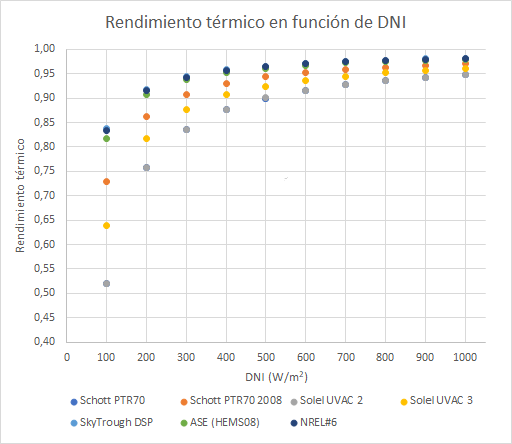
\includegraphics[width=0.9\linewidth]{images/resultados_test1a.png}
\caption{Rendimiento térmico en función de DNI para diferentes modelos de HCE} 
\label{fig:test1a}
\end{figure}

\subsection{Rendimiento del HCE en función de la temperatura de entrada}

\begin{table}[!h]
\centering
\caption{Rendimiento en función de la temperatura de entrada del HTF para diferentes modelos de HCE}
\label{tab:rendimiento_hce_tin}
\resizebox{\textwidth}{!}{%
\begin{tabular}{cccccccc}
\parbox{5em}{\centering $T_{in} (\circ C)$ } &
\parbox{5em}{\centering Schott  \\ PTR70} &
\parbox{5em}{\centering Schott  \\ PTR70 2008} &
\parbox{5em}{\centering Solel \\ UVAC 2} &
\parbox{5em}{\centering  Solel \\ UVAC 3} &
\parbox{5em}{\centering  SkyFuel \\ SkyTrough DSP} &
\parbox{5em}{\centering ASE\\ HEMS08} &
\parbox{5em}{\centering NREL\\ \#6} \\ \hline
473 & 0,975 & 0,986 & 0,974 & 0,982 & 0,993 & 0,993 & 0,993 \\
483 & 0,972 & 0,985 & 0,971 & 0,980 & 0,992 & 0,992 & 0,992 \\
493 & 0,969 & 0,983 & 0,969 & 0,978 & 0,991 & 0,990 & 0,991 \\
503 & 0,966 & 0,981 & 0,965 & 0,976 & 0,990 & 0,989 & 0,990 \\
513 & 0,963 & 0,979 & 0,962 & 0,973 & 0,988 & 0,988 & 0,988 \\
523 & 0,959 & 0,977 & 0,958 & 0,970 & 0,987 & 0,986 & 0,987 \\
533 & 0,955 & 0,975 & 0,955 & 0,967 & 0,986 & 0,984 & 0,985 \\
543 & 0,951 & 0,973 & 0,951 & 0,964 & 0,984 & 0,982 & 0,984 \\
553 & 0,946 & 0,970 & 0,946 & 0,960 & 0,982 & 0,980 & 0,982 \\
563 & 0,942 & 0,967 & 0,942 & 0,956 & 0,980 & 0,978 & 0,980 \\
573 & 0,937 & 0,964 & 0,937 & 0,952 & 0,978 & 0,976 & 0,978 \\
583 & 0,931 & 0,961 & 0,931 & 0,947 & 0,976 & 0,973 & 0,975 \\
593 & 0,925 & 0,957 & 0,926 & 0,943 & 0,974 & 0,970 & 0,973 \\
603 & 0,919 & 0,953 & 0,920 & 0,938 & 0,971 & 0,967 & 0,970 \\
613 & 0,912 & 0,949 & 0,914 & 0,932 & 0,968 & 0,963 & 0,967 \\
623 & 0,905 & 0,945 & 0,907 & 0,926 & 0,965 & 0,960 & 0,964 \\
633 & 0,898 & 0,941 & 0,900 & 0,920 & 0,962 & 0,956 & 0,961 \\
643 & 0,890 & 0,936 & 0,892 & 0,913 & 0,958 & 0,951 & 0,957 \\
653 & 0,881 & 0,931 & 0,884 & 0,906 & 0,955 & 0,947 & 0,954 \\
663 & 0,872 & 0,925 & 0,876 & 0,898 & 0,951 & 0,942 & 0,949 \\
673 & 0,863 & 0,919 & 0,867 & 0,890 & 0,946 & 0,937 & 0,945 \\
683 & 0,853 & 0,913 & 0,858 & 0,882 & 0,942 & 0,931 & 0,941
\end{tabular}%
}
\end{table}

\begin{figure}[!h]
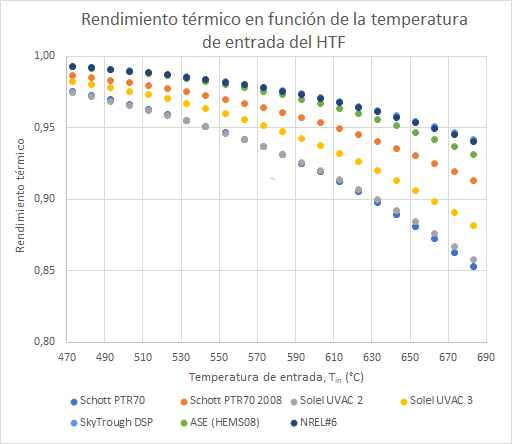
\includegraphics[width=0.9\linewidth]{images/resultados_test2a.png}
\caption{Rendimiento térmico en función de la temperatura de entrada del HTF para diferentes modelos de HCE} 
\label{fig:test2a}
\end{figure}



\subsection{Simulación con los diferentes modelos}

Comparamos ahora el resultado de simular con los tres modelos: modelo de 4º Orden, modelo de $1^{er}$ Orden y modelo simplificado. En las figuras puede verse el restultado para un día del año (se ha tomado el día 2 de marzo por tener buenas condiciones de radiación y estabilidad). 

\begin{table}[!h]
\centering
\caption{Temperaturas obtenidas en la simulación para cada modelo. Datos del día 2/3/2007. Condiciones estables y buena radiación}
\label{tab:temperaturas_modelos}
\resizebox{\textwidth}{!}{%
\begin{tabular}{ccccccc}
Hora &
\parbox{5em}{\centering DNI \\ $(W/m^2)$} &
\parbox{5em}{\centering $T_{in}$ \\ $(^\circ C)$} &
\parbox{5em}{\centering $T_{out}$  (SAM) \\ $(^\circ C)$} &
\parbox{5em}{\centering $T_{out}$ ($4^o Ord.$) \\ $(^\circ C)$} &
\parbox{5em}{\centering $T_{out}$  ($1^{er} Ord.$) \\ $(^\circ C)$} &
\parbox{5em}{\centering $T_{out}$ (Simplif.) \\  $(^\circ C)$}  \\ \hline
0:00  & 0   & 277 & 266 & 266 & 266 & 261 \\ 
1:00  & 0   & 273 & 262 & 262 & 262 & 258 \\
2:00  & 0   & 269 & 259 & 258 & 258 & 254 \\
3:00  & 0   & 265 & 255 & 255 & 255 & 251 \\
4:00  & 0   & 262 & 252 & 251 & 251 & 248 \\
5:00  & 0   & 258 & 249 & 248 & 248 & 245 \\
6:00  & 0   & 255 & 246 & 245 & 245 & 242 \\
7:00  & 234 & 252 & 263 & 243 & 243 & 240 \\
8:00  & 596 & 272 & 377 & 393 & 393 & 393 \\
9:00  & 724 & 292 & 392 & 393 & 393 & 393 \\
10:00 & 806 & 293 & 393 & 393 & 393 & 393 \\
11:00 & 859 & 293 & 393 & 393 & 393 & 393 \\
12:00 & 876 & 293 & 393 & 393 & 393 & 393 \\
13:00 & 867 & 293 & 393 & 393 & 393 & 393 \\
14:00 & 846 & 293 & 393 & 393 & 393 & 393 \\
15:00 & 781 & 293 & 393 & 393 & 393 & 393 \\
16:00 & 663 & 293 & 393 & 393 & 393 & 393 \\
17:00 & 420 & 293 & 313 & 281 & 281 & 275 \\
18:00 & 1   & 293 & 284 & 281 & 281 & 275 \\
19:00 & 0   & 298 & 282 & 285 & 285 & 280 \\
20:00 & 0   & 298 & 284 & 285 & 285 & 279 \\
21:00 & 0   & 293 & 281 & 281 & 281 & 276 \\
22:00 & 0   & 289 & 277 & 277 & 277 & 272 \\
23:00 & 0   & 284 & 273 & 273 & 273 & 268
\end{tabular}%
}
\end{table}

\begin{figure}[!h]
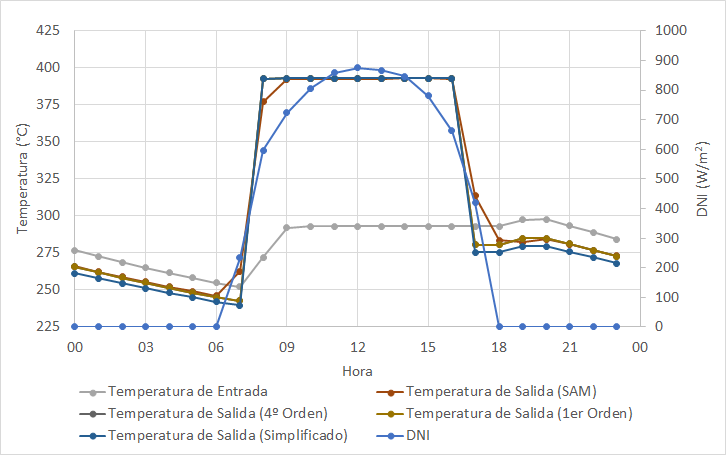
\includegraphics[width=0.9\linewidth]{images/temperaturas_modelos.png}
\caption{Temperaturas de salida obtenidas con los tres modelos} 
\label{fig:temperturas_modelos}
\end{figure}



\begin{table}[!h]
\centering
\caption{Caudales obtenidos en la simulación para cada modelo.  Datos del día 2/3/2007. Condiciones estables y buena radiación}
\label{tab:caudales_modelos}
\resizebox{\textwidth}{!}{%
\begin{tabular}{cccccc}
Hora &
\parbox{5em}{\centering DNI \\ $(W/m^2)$} &
\parbox{5em}{\centering Caudal  (SAM) \\ $(Kg/s)$} &
\parbox{5em}{\centering Caudal ($4^o Ord.$) \\ $(Kg/s)$} &
\parbox{5em}{\centering Caudal  ($1^{er} Ord.$) \\ $(Kg/s)$} &
\parbox{5em}{\centering Caudal (Simplif.) \\  $(Kg/s)$}  \\ \hline
0:00  & 0   & 204          & 204               & 204                & 204                   \\ 
1:00  & 0   & 204          & 204               & 204                & 204                   \\ 
2:00  & 0   & 204          & 204               & 204                & 204                   \\ 
3:00  & 0   & 204          & 204               & 204                & 204                   \\ 
4:00  & 0   & 204          & 204               & 204                & 204                   \\ 
5:00  & 0   & 204          & 204               & 204                & 204                   \\ 
6:00  & 0   & 204          & 204               & 204                & 204                   \\ 
7:00  & 234 & 204          & 204               & 204                & 204                   \\ 
8:00  & 596 & 530          & 514               & 516                & 518                   \\ 
9:00  & 724 & 660          & 669               & 670                & 672                   \\ 
10:00 & 806 & 648          & 661               & 663                & 664                   \\ 
11:00 & 859 & 614          & 630               & 632                & 634                   \\ 
12:00 & 876 & 599          & 617               & 619                & 621                   \\ 
13:00 & 867 & 632          & 648               & 650                & 651                   \\ 
14:00 & 846 & 699          & 714               & 716                & 718                   \\ 
15:00 & 781 & 736          & 750               & 752                & 753                   \\ 
16:00 & 663 & 599          & 620               & 622                & 624                   \\ 
17:00 & 420 & 204          & 204               & 204                & 204                   \\ 
18:00 & 1   & 204          & 204               & 204                & 204                   \\ 
19:00 & 0   & 204          & 204               & 204                & 204                   \\ 
20:00 & 0   & 204          & 204               & 204                & 204                   \\ 
21:00 & 0   & 204          & 204               & 204                & 204                   \\ 
22:00 & 0   & 204          & 204               & 204                & 204                   \\ 
23:00 & 0   & 204          & 204               & 204                & 204                   
\end{tabular}%
}
\end{table}

\begin{figure}[!h]
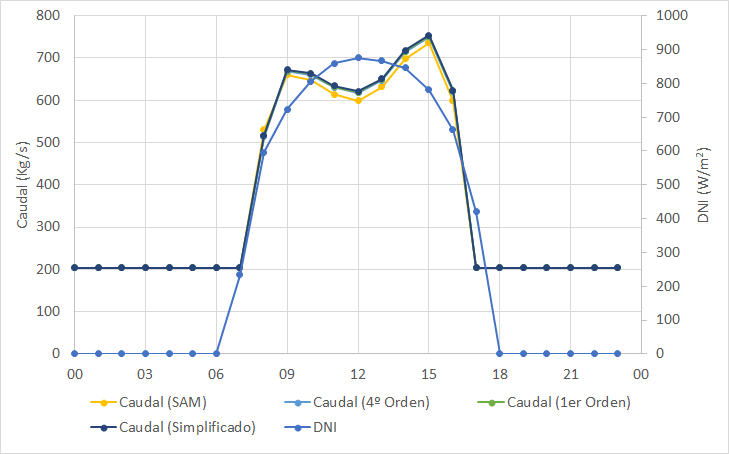
\includegraphics[width=0.9\linewidth]{images/caudales_modelos.png}
\caption{Caudales de salida obtenidos con los tres modelos} 
\label{fig:caudales_modelos}
\end{figure}


\begin{table}[!h]
\centering
\caption{Potencia térmica calculada en la simulación de cada modelo.  Datos del día 2/3/2007. Condiciones estables y buena radiación}
\label{tab:potencias_modelos}
\resizebox{\textwidth}{!}{%
\begin{tabular}{cccccc}
Hora &
\parbox{5em}{\centering DNI \\ $(W/m^2)$} &
\parbox{5em}{\centering $P_{th}$  (SAM) \\  $(MWt)$} &
\parbox{5em}{\centering $P_{th}$ ($4^o Ord.$) \\  $(MWt)$} &
\parbox{5em}{\centering $P_{th}$  ($1^{er} Ord.$) \\  $(MWt)$} &
\parbox{5em}{\centering $P_{th}$ (Simplif.) \\   $(MWt)$}  \\ \hline
0:00  & 0   & -4,9  & -5,0  & -5,0  & -6,9  \\
1:00  & 0   & -4,7  & -4,9  & -4,9  & -6,7  \\
2:00  & 0   & -4,5  & -4,8  & -4,8  & -6,5  \\
3:00  & 0   & -4,4  & -4,6  & -4,6  & -6,3  \\
4:00  & 0   & -4,2  & -4,5  & -4,5  & -6,0  \\
5:00  & 0   & -4,1  & -4,4  & -4,4  & -5,9  \\
6:00  & 0   & -3,9  & -4,3  & -4,3  & -5,7  \\
7:00  & 234 & 4,7   & -4,2  & -4,2  & -5,6  \\
8:00  & 596 & 133,1 & 149,5 & 150,1 & 150,5 \\
9:00  & 724 & 161,6 & 164,6 & 165,0 & 165,4 \\
10:00 & 806 & 157,7 & 161,2 & 161,6 & 162,1 \\
11:00 & 859 & 149,2 & 153,6 & 154,1 & 154,5 \\
12:00 & 876 & 145,5 & 150,5 & 150,9 & 151,3 \\
13:00 & 867 & 153,4 & 157,9 & 158,3 & 158,8 \\
14:00 & 846 & 170,2 & 174,2 & 174,6 & 175,0 \\
15:00 & 781 & 179,3 & 182,7 & 183,2 & 183,6 \\
16:00 & 663 & 145,6 & 151,1 & 151,6 & 152,0 \\
17:00 & 420 & 9,7   & -5,7  & -5,7  & -8,2  \\
18:00 & 1   & -4,4  & -5,7  & -5,7  & -8,1  \\
19:00 & 0   & -7,1  & -5,9  & -5,9  & -8,4  \\
20:00 & 0   & -6,3  & -5,9  & -5,9  & -8,4  \\
21:00 & 0   & -5,8  & -5,7  & -5,7  & -8,1  \\
22:00 & 0   & -5,5  & -5,5  & -5,5  & -7,8  \\
23:00 & 0   & -5,3  & -5,4  & -5,4  & -7,5 
\end{tabular}%
}
\end{table}


\begin{figure}[!h]
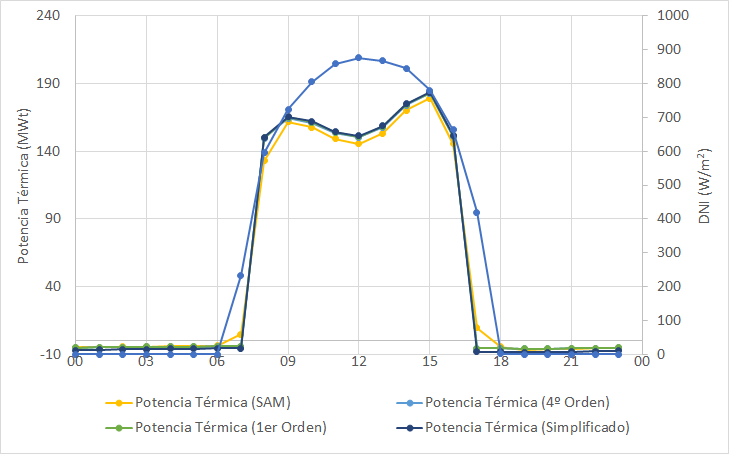
\includegraphics[width=0.9\linewidth]{images/potencias_modelos.png}
\caption{Potencia térmica obtenida con cada uno de los tres modelos} 
\label{fig:potencia_modelos}
\end{figure}


\begin{table}[!h]
\centering
\caption{Rendimientos obtenidos en la simulación de cada modelo.  Datos del día 2/3/2007. Condiciones estables y buena radiación}
\label{tab:rendimientos_modelos}
\resizebox{\textwidth}{!}{%
\begin{tabular}{ccccc}
Hora &
\parbox{5em}{\centering DNI \\ $(W/m^2)$} &
\parbox{5em}{\centering $\eta_{th}$ ($4^o Ord.$)} &
\parbox{5em}{\centering $\eta_{th}$  ($1^{er} Ord.$)} &
\parbox{5em}{\centering $\eta_{th}$ (Simplif.)} \\ \hline
0:00  & 0   & 0,000 & 0,000 & 0,000 \\
1:00  & 0   & 0,000 & 0,000 & 0,000 \\
2:00  & 0   & 0,000 & 0,000 & 0,000 \\
3:00  & 0   & 0,000 & 0,000 & 0,000 \\
4:00  & 0   & 0,000 & 0,000 & 0,000 \\
5:00  & 0   & 0,000 & 0,000 & 0,000 \\
6:00  & 0   & 0,000 & 0,000 & 0,000 \\
7:00  & 234 & 0,000 & 0,000 & 0,000 \\
 8:00  & 596 & 0,912 & 0,917 & 0,920 \\
9:00  & 724 & 0,916 & 0,920 & 0,922 \\
10:00 & 806 & 0,914 & 0,918 & 0,920 \\
11:00 & 859 & 0,910 & 0,914 & 0,917 \\
12:00 & 876 & 0,909 & 0,912 & 0,915 \\
13:00 & 867 & 0,913 & 0,916 & 0,919 \\
14:00 & 846 & 0,920 & 0,923 & 0,926 \\
15:00 & 781 & 0,923 & 0,926 & 0,928 \\
16:00 & 663 & 0,907 & 0,911 & 0,914 \\
17:00 & 420 & 0,000 & 0,000 & 0,000 \\
18:00 & 1   & 0,000 & 0,000 & 0,000 \\
19:00 & 0   & 0,000 & 0,000 & 0,000 \\
20:00 & 0   & 0,000 & 0,000 & 0,000 \\
21:00 & 0   & 0,000 & 0,000 & 0,000 \\
22:00 & 0   & 0,000 & 0,000 & 0,000 \\
23:00 & 0   & 0,000 & 0,000 & 0,000
\end{tabular}%
}
\end{table}

\begin{figure}[!h]
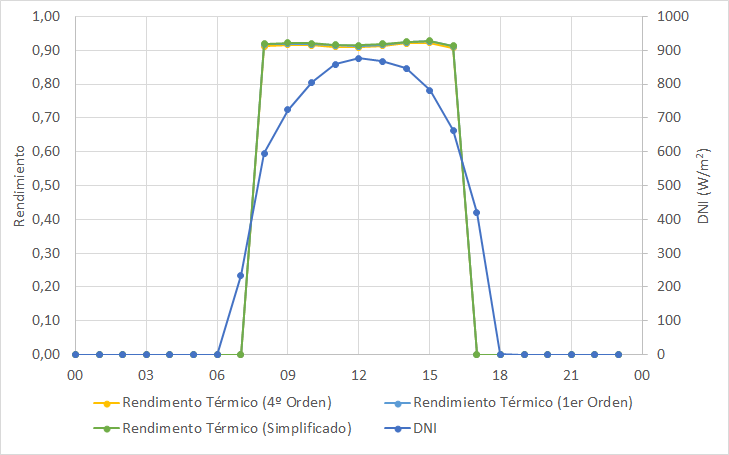
\includegraphics[width=0.9\linewidth]{images/rendimientos_modelos.png}
\caption{Rendimiento térmico para cada uno de los tres modelos} 
\label{fig:rendimientos_modelos}
\end{figure}

\subsection{Simulación cambiando el tamaño de la malla de integración}
\label{mallaintegracion}


\begin{figure}[!h]
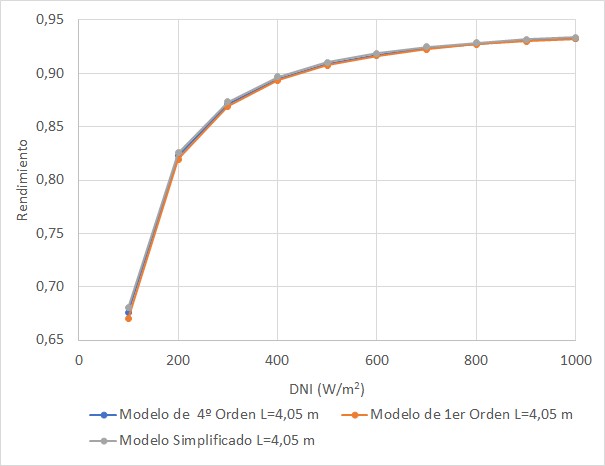
\includegraphics[width=0.9\linewidth]{images/malla0405.png}
\caption{Rendimiento calculado con cada modelo para un tamaño de malla de integración de 4,05 m} 
\label{fig:malla0405}
\end{figure}

\begin{figure}[!h]
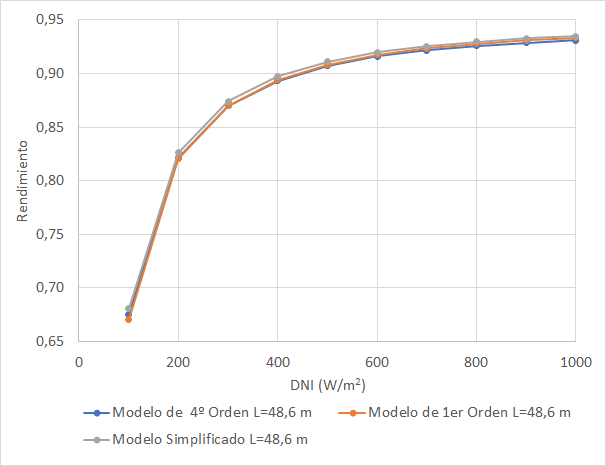
\includegraphics[width=0.9\linewidth]{images/malla4860.png}
\caption{Rendimiento calculado con cada modelo para un tamaño de malla de integración de 48,60 m} 
\label{fig:malla4860}
\end{figure}

\begin{figure}[!h]
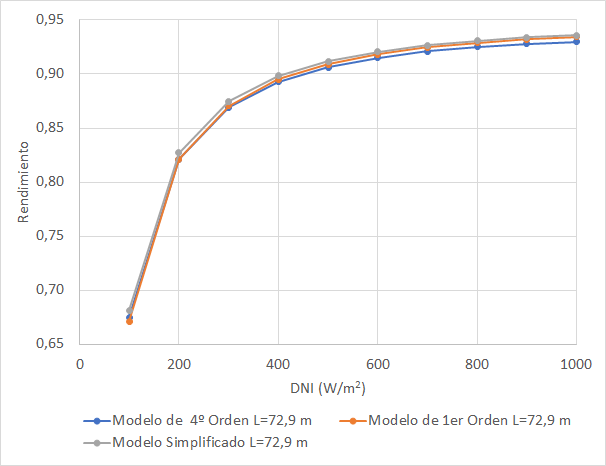
\includegraphics[width=0.9\linewidth]{images/malla7290.png}
\caption{Rendimiento calculado con cada modelo para un tamaño de malla de integración de 72,90 m} 
\label{fig:malla7290}
\end{figure}

\begin{figure}[!h]
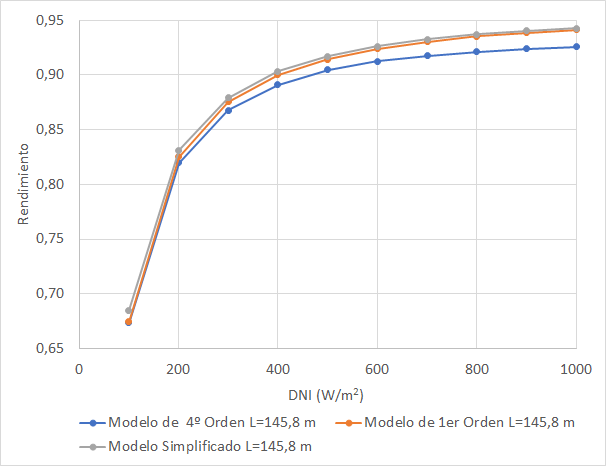
\includegraphics[width=0.9\linewidth]{images/malla14580.png}
\caption{Rendimiento calculado con cada modelo para un tamaño de malla de integración de 145,80 m} 
\label{fig:malla14580}
\end{figure}



\begin{figure}[!h]
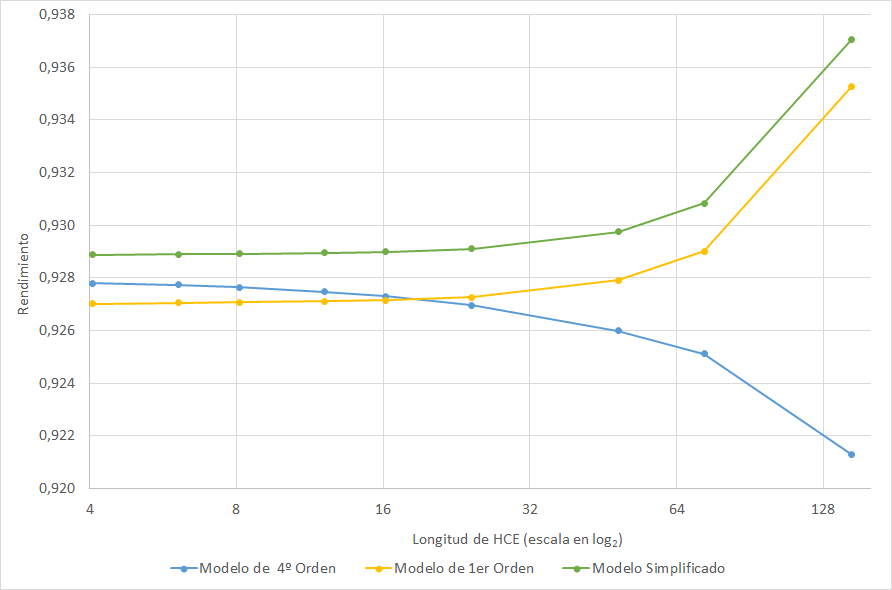
\includegraphics[width=0.9\linewidth]{images/malla_variable_DNI_800.png}
\caption{Rendimiento calculado para diferentes tamaños de malla de integración. $DNI=800 W/m^2$, $T_{in}=300 \circ C$, $\dot m = 6 kg/s$} 
\label{fig:malla_variable_DNI_800}
\end{figure}






